\chapter{Modelling the Floral Transition}% in Arabidopsis
\label{chapter:flowering}
\section{Introduction}

The initiation of the floral transition is a key decision during plant development.
Diverse species have evolved to respond to environmental cues to flower in the correct season.
Despite these specific differences key properties such as irreversibility and robustness to fluctuating signals appear to be conserved in individual meristems of monocarpic annuals.
In Arabidopsis many genes have been discovered and placed in regulatory networks without considering the specific temporal or spatial effect this could have on the network properties.
This motivates a dynamic model of known regulators to help us gain an understanding of how genetic interactions can lead to morphological change over time.
In this chapter we will use mathematical modelling to understand the essential properties of the transition.
Our models will be placed on quantitative foundations with the aim of capturing some of the underlying biology in a developing plant system.
The models will be trained using leaf number data from various genotypes perturbed for key genes that regulate the vegetative to floral transition and predictions made for others.
The use of linear models will be explored and then a demonstration of how small regulatory networks of core components are sufficient to capture the dynamic behaviour of the floral transition.
The mathematical assumptions and simplifications will be clearly stated and the models described in detail.
The value of pursuing an iterative approach combining modelling with experimental work to capture key features of complex systems will be highlighted.
Nested sampling, as described in \autoref{chapter:nestedSampling}, will be used to place the models in a Bayesian context thus giving robust statistical treatment of the problems being addressed.
Nested sampling will be used for parameter inference and for comparison of models of the floral transition developed in this chapter.
Using the Bayesian framework allows further information to be used as it becomes available and possible avenues for taking this work forward are discussed along with a detailed critique of the models developed.

\section{Initial considerations}
\subsection{Hubs}

In Arabidopsis many genetic studies have revealed major components of gene regulatory networks.
From these experiments it has been found that the entire network of flowering time control is highly complex with many interacting signals and pathways~\cite{turck2008,higgins2010}.
This complexity coupled with a lack of kinetic parameter data can lead to models that are highly underconstrained by the available biological data.
Thus an appropriate way of tackling such a large system is to consider a reductionist approach.
The motivation for reducing the complexity is that it is easier to work with a reduced number of variables and parameters but can still provide insights into the biology.
One way of reducing such a large system is to take advantage of some genetic redundancy in the plant and approximate key genes for entire hub activities.
This is not an uncommon approach in the literature when tackling redundancy (for example see van Mourik et al.~\cite{vanmourik2010}).
Therefore an initial simplification for this chapter is to group genes with similar effects into distinct hubs or functional modules~\cite{alon2006}.

By doing this early in our analysis we will lose a direct mapping onto individual genes yet, as we have phenotypic data available for transgenic or mutant lines perturbed for the major genes controlling the hubs, we can still relate back to biological units.
Simplifying the known flowering regulatory network as a set of key hubs has the advantage of making it potentially easier to identify the critical network interactions that account for the major behaviours of the system.
As an example, mutations in both \emph{FD} and its paralogue \emph{FDP} have been shown to cause later flowering phenotypes than either individually and the double mutant significantly reduces the effect of \emph{FT} overexpression~\cite{jaeger2013} (see also \autoref{tab:data}).
These two closely related genes can therefore be grouped together in to a single hub, named after its major contributor, FD.
Another example would be the AP1 hub that would also include CAL, which is partially redundant with AP1~\cite{bowman1993}.
Double mutants in these genes have curious cauliflower-like inflorescences~\cite{gustafson1994,ferrandiz2000}.
The FT hub would also include the activity of its close relative TSF~\cite{yamaguchi2005}.
As discussed in \autoref{sec:ftGenetics} LFY is a master integrator that functions in multiple pathways so it makes sense that this will provide a hub.
Finally we include a hub that can antagonise the floral transition and promote meristem identity.
This is named after TFL1 --- a key floral repressor.
In total the whole flowering regulation network is simplified down into five hubs labelled after their major constituents: FT, TFL1, FD, LFY and AP1.
The AP1 hub is used as the output in the modelling work presented here as its upregulation is known to be an early indicator of the floral transition in Arabidopsis~\cite{mandel1992,wigge2005}.

\subsection{Data}

The quantitative data used in this study were provided by Phil Wigge and Katja Jaeger who grew 16 plant genotypes and measured their rosette and cauline leaf numbers.
These data are provided in \autoref{tab:data} including various mutant and overexpressing transgenic lines under the control of the cauliflower mosaic virus 35S promoter (35S).
To validate the models and predictions in terms of leaf numbers this data set was divided into a training set and a prediction set.
Although the data are not independent, because a number of combinations of genes are present or absent in multiple genotypes, an appropriate way to assign to these subsets was to predict the triple mutant leaf numbers.
This would also be a significant and challenging test of the models' predictive capacity because of the unknown combinatorial effects of the gene interactions.

\begin{table*}[!htb]
\centering
\setlength{\tabcolsep}{3pt}
\begin{tabular}{@{}l@{\hspace{-1em}}cccccc@{}}
%      \begin{tabular}{@{}l@{}cp{6em}p{6em}ccc@{}}
    %\begin{tabularx}{\textwidth}{@{}l*{5}{>{\centering\arraybackslash}X}c@{}}
  \toprule%
  Genotype & No. of plants & \parbox[c]{6em}{\centering Number of \\ \vspace{-0.7ex}rosette leaves\vphantom{$k_j$} } & \parbox[c]{6em}{\centering Number of \\\vspace{-0.7ex}cauline leaves\vphantom{$k_j$}} & Total leaves & SD of total & Data set \\
      \toprule%
      Wildtype (Col)               & 12 & 7.9   & 1.4   & 9.3   & 1.1  & Training\\
      35S:\emph{FT}                & 10 & 4.4   & 1.0   & 5.4   & 0.7  & Training\\ 
      35S:\emph{LFY}               & 11 & 3.8   & 1.8   & 5.6   & 0.8  & Training\\
      35S:\emph{TFL1}              & 12 & 27.5  & 15.7  & 43.2  & 1.9  & Training\\
      \emph{lfy-12}                & 9  & 13.0  & 5.3   & 18.3  & 1.2  & Training\\
      \emph{ft-10}                 & 10 & 36.4  & 9.3   & 45.7  & 1.3  & Training\\
      \emph{tfl1-1}                & 11 & 7.7   & 0.4   & 8.1   & 0.8  & Training\\
      \emph{fd-2}                  & 12 & 18.5  & 4.63  & 23.13 & 2.47 & Training\\
      \emph{fdp-1}                 & 10 & 11.2  & 2.0   & 13.2  & 1.3  & Training\\
      \emph{fd-2 fdp-1}            & 10 & 32.9  & 6.3   & 39.2  & 1.1  & Training \\
      35S:\emph{TFL1 fd-2}         & 12 & 23.8  & 8.2   & 32.0  & 2.1  & Training \\
      \emph{tfl1-1 fd-2}           & 12 & 14.4  & 4.6   & 19.0  & 1.2  & Training \\
      35S:\emph{FT fd-2}           & 12 & 8.3   & 2.4   & 10.7  & 1.35 & Training \\
      \emph{tfl1-1 fd-2 fdp-1}     & 12 & 24.83 & 6.67  & 31.5  & 1.38 & Prediction \\
      35S:\emph{TFL1 fd-2 fdp-1}   & 10 & 31.33 & 11.0  & 42.33 & 2.89 & Prediction \\
      35S:\emph{FT fd-2 fdp-1}     & 12 & 25.8  & 5.6   & 31.4  & 1.34 & Prediction \\
      \bottomrule%
    \end{tabular}
    \caption{Experimental leaf number data.
      For each genotype the table lists the mean of the experimental data for rosette and cauline leaves, total leaf number (TLN) and the calculated standard deviation (SD) of the TLN.
      The wildtype and all single and double mutant data comprised the model training set for parameter inference.
      The triple mutant data are predicted using the inferred parameters from the training phase.}
    \label{tab:data}
\end{table*}

\subsection{Linear modelling}

Initially we consider a QTL-type approach for capturing the total leaf number data in terms of a number of genes involved in the floral transition.
In QTL studies a single-marker analysis is the simplest conceptual method of detecting a QTL and can be conducted with statistical tests such as ANOVA or a t-test depending on how the population was crossed.
Performing a linear regression is also a simple and common way of analysing traits of interest.
This method was chosen for the present study because we don't have a mapping population and data set as would be considered in a traditional QTL analysis.
Thus a simple linear summation of relative estimated gene expression levels was utilised.
This linear model takes a combination of the concentrations (where necessary denoted with square brackets) of FT, TFL1, FD and LFY, plus an intercept term which would represent the population mean in a QTL study.
AP1 is not included as we use this as a proxy for the leaf number data which is the output of the model (discussed in more detail in \autoref{sec:scaling}) and \emph{AP1} mutant genotypes were not available.
Thus the linear model can simply be stated as
\begin{equation*}
\text{Total leaf numbers} = k_1 + k_2[FT] + k_3[TFL1] + k_4[FD] + k_5[LFY]
\end{equation*}
which is a five parameter linear regression problem with $k_i$ being the constants to estimate.
Genotypes were assigned weights for each gene depending on the contribution of mutating or overexpressing the genes.
The wildtype gene was assigned a value of 1; full knockouts were assigned 0; 35S overexpressors were assigned 10 to reflect the massive ectopic expression; and the \emph{fd-2} and \emph{fdp-1} mutations had levels of 0.25 and 0.8 respectively to approximately reflect their \emph{in planta} partial knockout effect.
These values were chosen because the \emph{fd-2} mutant clearly has a stronger effect on flowering time than \emph{fdp-1} (\autoref{tab:data}) but in combination are far more potent.
Thus full FD hub mutants (in the models in this thesis represented by the data from \emph{fd-2 fdp-1}) have a total weight of 0.05.
It is not expected that these choices are particularly important due to the number of free parameters in the model that can adjust for any differences in these values.

Nested sampling was used to estimate the parameters and evidence of the linear model initially by using the known standard deviation in the total leaf numbers to place a different normal distribution on each data point.
The log-evidence was worse than $-11000$ strongly indicating that the variation in the leaf number data could not be captured by this model.
Indeed, plotting the posterior mean and standard deviations of the leaf numbers for each genotype against the true leaf numbers reveals that many genotypes are poorly estimated, as shown in \autoref{fig:FTlinearIndSig}.
\begin{figure}[!htbp]
\centering
\includegraphics[height=0.45\textheight]{/home/nick/Dropbox/march2014/multinest4thesis/FTlinearModellingIndSigma/FTlinearIndSig.pdf}
\sidecaption[][-290pt]{Fit of a linear model with independent errors in the data of each genotype.
The general trend may be broadly correct yet this model is not particularly accurate.
The tiny error bars (representing one standard deviation) of the estimated leaf numbers indicate a lack of flexibility in the parameters that maximise the likelihood function.
One genotype, \emph{35S:FT}, was estimated to have negative leaf numbers, but this could be controlled for with further constraints.
\label{fig:FTlinearIndSig}}
\end{figure}
If the model fitted perfectly the points would all fall on to the dark line.
The small estimated standard deviations suggest the mean parameter values are the ones which maximise the likelihood function with little room for variation in those values.
Note that, without further constraints, the \emph{35S:FT} genotype is estimated to have negative leaf numbers which is obviously not biologically possible.

To try to alleviate the issues with the constraints on the data an extra parameter for the error term in the data set was added.
Thus now all data points share the same standard deviation term which follows a Jeffreys-type prior (as the standard deviation is a scale parameter)~\cite{jeffreys1961}, rather than their associated individual standard deviations.
This results in a log-evidence of $-69.85\pm 0.13$.
An equivalent plot as before is shown in \autoref{fig:FTlinear}.
\begin{figure}[!htbp]
\centering
\includegraphics[height=0.45\textheight]{/home/nick/Dropbox/march2014/multinest4thesis/FTlinearModelling/FTlinear.pdf}
\sidecaption[][-290pt]{Fit of a linear model with the error model variance inferred as a parameter and individual standard deviations not considered.
The estimates and predictions are slightly better than in \autoref{fig:FTlinearIndSig}.
Our error bars are much more in line with the experimental error bars than previously.
The predicted mean estimate of \emph{35S:TFL1 fd-2 fdp-1} is almost exactly correct.
\label{fig:FTlinear}}
\end{figure}
This plot was constructed by taking the 1000 highest likelihood samples from the posterior set to reduce the influence of the inferred variance parameter affecting the likelihood.
In other words by doing this it is expected that a good likelihood fit is more likely due to the parameters of interest themselves rather than the parameter controlling the variance in the error model.
The standard deviations of the resulting estimated leaf numbers are now on a similar level to the true data in a number of cases.
Our predicted triple mutants are improved overall with \emph{35S:TFL1 fd-2 fdp-1} being remarkably close to the experimental result although \emph{35S:FT fd-2 fdp-1} is predicted to have 20 leaves fewer than in reality.

Running the linear model in this way is identical to calculating a least-squares regression.
These regression statistics were confirmed using \texttt{R}'s \cite{Rcoreteam} linear model function \texttt{lm()} which produced similar estimates for the parameters.
As a side note the computed Adjusted R-squared value suggests we explain 29\% of the variability in the data with this linear model.
The estimated against true total leaf numbers for all models considered here are shown in \autoref{tab:lmLeafNums}.
\begin{table*}[!htbp]
\setlength{\tabcolsep}{5pt}
    \begin{tabular}{@{}lcccccccc@{}}
      \toprule%
      Genotype & \multicolumn{4}{c}{Mean total leaves} & \multicolumn{3}{c}{SD of total leaves} & Data set \\
      \cmidrule(r){2-5} \cmidrule{6-8}
      & True & Ind. $\sigma$ & Inferred $\sigma$ & \texttt{R lm()} & True & Ind. $\sigma$ & Inferred $\sigma$ \\
%      \toprule%
%      Genotype & \multicolumn{4}{c}{Mean total leaves} & \multicolumn{3}{c}{SD of total leaves} & Model set \\
%      \cmidrule(r){2-5} \cmidrule{6-8}
%      & True & Independent $\sigma$ & One $\sigma$ & \texttt{R lm()} & True & Independent $\sigma$ & One $\sigma$ \\
      \toprule%
      Wildtype (Col)             & 9.3   & 13.5 & 19.7 & 19.8 & 1.1  & 0.07 & 2.5 & Training\\
      35S:\emph{FT}              & 5.4   & -4.6 & 4.4  & 4.1  & 0.7  & 0.23 & 4.8 & Training\\ 
      35S:\emph{LFY}             & 5.6   & 5.0  & 6.3  & 5.9  & 0.8  & 0.22 & 6.1 & Training\\
      35S:\emph{TFL1}            & 43.2  & 39.6 & 35.6 & 35.7 & 1.9  & 0.46 & 4.6 & Training\\
      \emph{lfy-12}              & 18.3  & 14.5 & 21.2 & 21.3 & 1.2  & 0.08 & 2.8 & Training\\
      \emph{ft-10}               & 45.7  & 15.5 & 21.4 & 21.5 & 1.3  & 0.08 & 2.7 & Training\\
      \emph{tfl1-1}              & 8.1   & 10.6 & 17.9 & 18.0 & 0.8  & 0.09 & 2.7 & Training\\
      \emph{fd-2}                & 23.13 & 31.5 & 25.1 & 25.1 & 2.47 & 0.07 & 2.7 & Training\\
      \emph{fdp-1}               & 13.2  & 18.3 & 21.1 & 21.2 & 1.3  & 0.06 & 2.1 & Training\\
      \emph{fd-2 fdp-1}          & 39.2  & 36.4 & 26.6 & 26.5 & 1.1  & 0.09 & 3.4 & Training \\
      35S:\emph{TFL1 fd-2}       & 32.0  & 57.6 & 41.1 & 41.0 & 2.1  & 0.46 & 4.6 & Training \\
      \emph{tfl1-1 fd-2}         & 19.0  & 28.6 & 23.4 & 23.3 & 1.2  & 0.08 & 2.9 & Training \\
      35S:\emph{FT fd-2}         & 10.7  & 13.4 & 9.8  & 9.4  & 1.35 & 0.23 & 4.7 & Training \\
      \emph{tfl1-1 fd-2 fdp-1}   & 31.5  & 33.5 & 24.8 & 24.7 & 1.38 & 0.10 & 3.6 & Prediction \\
      35S:\emph{TFL1 fd-2 fdp-1} & 42.33 & 62.4 & 42.5 & 42.5 & 2.89 & 0.46 & 5.1 & Prediction \\
      35S:\emph{FT fd-2 fdp-1}   & 31.4  & 18.2 & 11.3 & 10.8 & 1.34 & 0.23 & 5.1 & Prediction \\
      \bottomrule%
    \end{tabular}
    \caption{Experimental and linear model leaf numbers. For each genotype the table lists the mean true experimental total leaf numbers and standard deviations (SD) together with those estimated (for the training set) or predicted using the linear models described in the text.
      \texttt{R}'s \texttt{lm()} function does not produce an uncertainty estimate.
      Ind., Independent i.e\@. the case where each genotype's SD was used in the likelihood function.
    }
    \label{tab:lmLeafNums}
\end{table*}

Taken together these results suggest that for this small system and for the given data a linear modelling approach is limited in its accuracy.
Specifically it was shown that a linear model gives estimates that are too inaccurate to capture the underlying biology without further constraints.
QTL-type linear modelling has a value due to its simplicity especially for genome-wide data and where there are a large number of lines available to be scored.
For this data set and simplified hub model however, this approach does not appear flexible enough to be appropriate.
Thus in the rest of this chapter a more detailed mechanistic approach is constructed based on an ODE model that can provide better leaf number predictions, trace the dynamics of a developing system, capture key properties of the floral transition and lead to interesting predictions that can be tested experimentally.
However, this flexibility requires far more parameters and a much greater investment in computer time.

\subsection{Simple networks}\label{sec:simpleNets}
\subsubsection{Introduction}

For a number of species, homologues of the Arabidopsis master regulator FT are a core element of the photoperiod pathway~\cite{higgins2010,tamaki2007}.
In Arabidopsis diurnal \emph{CO} activity gives rise, in long days, to stable CO which upregulates \emph{FT}~\cite{samach2000,valverde2004}.
Long range signalling of FT promotes flowering time~\cite{corbesier2007,mathieu2007,jaeger2007}, thus oscillating input signals are interpreted at some level and, once in a floral primordium, the cells are committed to transition.
This section presents a simple demonstration of how two of the important properties of the floral transition, namely noise-filtering and irreversibility, can be exhibited by simple three node networks in feedforward loops.
The nodes consist of the complex FT with FD, and the floral transcription factors LFY and AP1.
Although labelled for the Arabidopsis genes, the qualitative effects of the motifs apply equally well to other species.

A set of ODEs is used to describe the dynamic behaviour of the system and numerically solved.
Binary step functions are used for the transcriptional activation of genes and AND, OR or AND/OR gating, depending on the network.
The equations all follow the standard form of
\begin{equation*}
\frac{dx}{dt}= \nu - \delta x, \text{ for } x\in \{LFY,AP1\},
\end{equation*}
where $\nu$ is the transcription term and $\delta$ the degradation rate.
The FT input signal to the system in this section was modelled as a digital function, either 0 or 1.
In these examples a signal of long duration and a small blip are used which might represent, for example, a one-off short exposure to sunlight.
All initial conditions are set to $0$ and parameters fixed.

\subsubsection{The Coherent Feedforward Loop}

\begin{figure*}[!htb]
\centering
\begin{subfigure}[b]{0.43\linewidth}
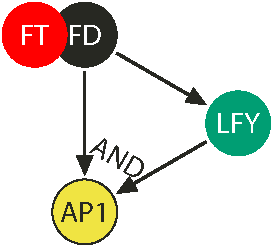
\includegraphics[width=\linewidth,page=1]{/home/nick/Dropbox/thesis/loops.pdf}
\caption{
This motif is very common in \emph{Escherichia coli}, yeast and other organisms~\cite{mangan2003}.
It has been referred to as a sign-sensitive delay element because it has a delayed on response but immediate off response~\cite{alon2006}.
}
\label{fig:cohFFL}
\end{subfigure}
\begin{subfigure}[b]{0.56\linewidth}
\includegraphics[width=\linewidth]{/home/nick/Dropbox/march2014/multinest4thesis/simpleNets/FFloopsCOH.pdf}
\caption{%Noise filtering by the coherent feedforward loop.
Responses of LFY (green) and AP1 (yellow) to a short and a long incoming FT signal (purple) are shown.
The short pulse in filtered out and the longer signal leads to (delayed) activation of AP1.
Decay in response to a fall in FT is immediate.
}
\label{fig:cohFFLdyn}
\end{subfigure}
\captionsetup{justification=centering}
\caption{The coherent feedforward loop and its dynamics.}%\label{}
\end{figure*}

The coherent feedforward loop is a network motif that is commonly found in signalling networks~\cite{mangan2003, alon2006}.
One node regulates another, with both jointly regulating a third, \autoref{fig:cohFFL}.
If the joint regulation is with an AND logic gate this simple network has persistence detection and thus is able to be used as a noise filter that removes blips in a signal.
As the correct timing of the floral transition is crucial to reproductive success it is important that the system integrates information over time, and is not incorrectly activated by noise~\cite{hasty2000}.

In the equations below we write $\theta_{FT.LFY} (FT)$ (where $\theta$ represents a Heaviside step-function) to mean that when FT is greater than (or equal to) the threshold at which it binds to the promoter site of \emph{LFY}, FT activates \emph{LFY} transcription.
Similarly $\theta_{FT.AP1} (FT)$ means \emph{AP1} is activated when FT is greater than or equal to the \emph{AP1} promoter-binding threshold.
The threshold for the activation of \emph{LFY} and \emph{AP1} is set at $\mathrm{FT}=1$.
$\theta_{LFY.AP1} (LFY)$ means that when LFY reaches a threshold, here 0.5, it binds the \emph{AP1} promoter and thus activates \emph{AP1} transcription.
The activation constants, $\nu$, and degradation constants, $\delta$, were set to 1 to scale the results to be maximally 1.
The equations for this system are therefore as follows
\begin{equation*}
\dd{LFY}{t} = \nu_{LFY} \theta_{FT.LFY} (FT) -\delta_{LFY} LFY,
\end{equation*}
\begin{equation*}
\dd{AP1}{t} = \nu_{AP1} \theta_{FT.AP1} (FT)\theta_{LFY.AP1} \left(LFY\right) -\delta_{AP1} AP1.
\end{equation*}

The dynamics of this network are shown in \autoref{fig:cohFFLdyn}.
This network motif has been described previously and has been shown to exhibit noise filtering properties for short bursts of the incoming signal that are below the delay time through the different routes in the pathway~\cite{mangan2003,alon2006}.
This is clearly seen in the figure where the short pulse of signal is filtered out whereas the longer signal is transferred through the network.
By introducing an arbitrary threshold for flowering, seen in the lower AP1 panel of \autoref{fig:cohFFLdyn}, this network shows a reversion to a non-flowering state after FT decay.

\subsubsection{The Regulated Feedforward Loop}

\begin{figure*}[!htb]
\centering
\begin{subfigure}[b]{0.42\linewidth}
\includegraphics[width=\linewidth,page=2]{/home/nick/Dropbox/thesis/loops.pdf}
\caption{
This motif is often found in developmental transcription networks~\cite{mangan2003}.
The feedback between the two targets of the first node can cause a memory effect as they keep active even in the absence of a signal from the initial regulator~\cite{alon2006}.
}
\label{fig:regFFL}
\end{subfigure}
\begin{subfigure}[b]{0.57\linewidth}
\includegraphics[width=\linewidth]{/home/nick/Dropbox/march2014/multinest4thesis/simpleNets/FFloopsREG.pdf}
\caption{%Memory created by the regulated feedforward loop.
Responses of LFY (green) and AP1 (yellow) to a short and a long incoming FT signal (purple) are shown.
The short blip leads to a small rise in LFY and AP1 levels but not enough to be maintained.
The long signal induces both targets enough so that when FT drops away the double-positive feedback loop maintains both LFY and AP1.
}
\label{fig:regFFLdyn}
\end{subfigure}
\captionsetup{justification=centering}
\caption{The regulated feedforward loop and its dynamics.}%\label{}
\end{figure*}

A similar three node network, called regulated feedforward or double-positive feedback~\cite{alon2006}, that uses an OR logic gating can exhibit irreversibility.
With the same nodes, an extra activating connection between the two targets of the first complex will mean the targets are mutually activating given enough initial impulse by the first (\autoref{fig:regFFL}).
If these conditions are met the network can provide memory of the input signal.
This is important in developmental networks because they operate on slower timescales than sensory networks.
For example commitment to flowering after exposure to long days has been shown to take 1--7 days depending on plant age and seed vernalization treatment~\cite{corbesier1996} whereas a sensory response in the shoot to salt stress in the root has been shown to take in the order of minutes, propagated in part by a rapid calcium wave~\cite{choi2014}.
%such as leaflet closure in the touch-me-not plant, \emph{Mimosa pudica}, is in the order of minutes in response to change of light conditions~\cite{burkholder1936}.
%Furthermore responses of some species to touch are well known to be in the order of seconds.
%The well studied example of the Venus fly trap, \emph{Dionaea muscipula}, shuts its trap within a second and the aforementioned \emph{M. pudica} responds to mechanical stimulation by closing its leaflets very rapidly (both reviewed by Braam~\cite{braam2005}).

The notation of the equations for this loop is identical to that for the coherent feedforward loop.
There is an additional connection in this network as shown in \autoref{fig:regFFL}.
This is controlled by the term $\theta_{AP1.LFY} (AP1)$ which means that when AP1 is greater than or equal to the threshold at which it binds to the promoter site of \emph{LFY}, AP1 activates \emph{LFY} transcription.
Both thresholds between LFY binding \emph{AP1} and vice versa were set at values of 0.45.
This creates the double-positive feedback loop~\cite{alon2006}.
Due to using OR logic gating, rather than AND logic, the equations take the higher of whichever activator is bound, leading to

\begin{equation*}
\dd{LFY}{t} = \nu_{LFY}\max\left(\theta_{FT.LFY} (FT),\theta_{AP1.LFY} (AP1)\right) - \delta_{LFY}LFY,
\end{equation*}
\begin{equation*}
\dd{AP1}{t} = \nu_{AP1}\max\left(\theta_{FT.AP1} (FT),\theta_{LFY.AP1} (LFY)\right) - \delta_{AP1}AP1.
\end{equation*}

The dynamics of this motif are shown in \autoref{fig:regFFLdyn}.
Once LFY reaches a concentration level that can activate \emph{AP1}, this interaction is sufficient to maintain AP1 production even in the absence of the incoming signal FT.
If the FT signal is removed before LFY has accumulated to a sufficient level then AP1 will degrade away before floral commitment.
The network therefore shows a memory effect and irreversibility~\cite{alon2006}.
With the arbitrary threshold for flowering, seen in the lower AP1 panel of \autoref{fig:regFFLdyn}, the double-positive feedback shows maintenance of a flowering state even after FT decay.

\subsubsection{A Compromise Feedforward Loop}

\begin{figure*}[!htb]
\centering
\begin{subfigure}[b]{0.42\linewidth}
\includegraphics[width=\linewidth, page=3]{/home/nick/Dropbox/thesis/loops.pdf}
\caption{
This network incorporates the two previous motifs by utilising different transcription rates.
A low rate requires the presence of only one signal employing an OR gate.
A higher rate of transcription can be achieved by both regulators being present so using an AND gate.
We get some noise filtering and a partial memory effect.
}
\label{fig:compFFL}
\end{subfigure}
\begin{subfigure}[b]{0.56\linewidth}
\includegraphics[width=\linewidth]{/home/nick/Dropbox/march2014/multinest4thesis/simpleNets/FFloopsCOMP.pdf}
\caption{%A compromise feedforward loop shows some noise-filtering and memory effect.
Responses of LFY (green) and AP1 (yellow) to a short and a long incoming FT signal (purple) are shown.
The blip in FT causes a damped response by both genes.
Past a threshold during the longer signal the AND gate will be switched on enabling a higher rate of transcription.
As the signal abates the transcription rate is reduced to the lower level but this is still at or above an introduced threshold for flowering.
}
\label{fig:compFFLdyn}
\end{subfigure}
\captionsetup{justification=centering}
\caption{A compromise feedforward loop and its dynamics.}%\label{}
\end{figure*}

While the previous two simple network motifs capture separate characteristics of the floral transition, in order to reproduce both noise filtering and irreversibility within the same network the logic gating rules require an extension.
This can be achieved by introducing two transcription rates, a low rate that can be activated by either FT or LFY and a higher rate that requires the presence of both FT and LFY (\autoref{fig:compFFL})
\sidenote[][-18pt]{\emph{Espinosa-Soto et al.~\cite{espinosa2004}  have used a similar idea. % in their discrete network. 
An intermediate level of expression is determined from experimental data for a number of nodes. This, as here, allows for different activation thresholds.}}%[-100pt]
.
Hence we combine the key features of both previous network motifs by using two different levels of activation depending on the number of activators bound.
The logic gating uses OR for transcriptional activation at a reduced level but requires AND for maximal activation.
The higher levels, $\nu_{LFY,1}$ and $\nu_{AP1,1}$, are set to 1, and the lower levels, $\nu_{LFY,2}$ and $\nu_{AP1,2}$, are set to 0.5.
These ideas lead to the following equations:
\begin{equation*}
\dd{LFY}{t}  =
  \begin{cases} 
\nu_{LFY,1} - \delta_{LFY}LFY & 
    \begin{aligned}[c]
       & \text{if }\theta_{FT.LFY}\left(FT\right)=1 \text{ and } \\
       & \theta_{AP1.LFY} \left(AP1\right) =1
    \end{aligned}   \\[1ex]
\!\begin{aligned}[c]
       & \nu_{LFY,2} \max\left(\theta_{FT.LFY} \left(FT\right),\theta_{AP1.LFY}
  \left(AP1\right)\right)\\
& \phantom{\nu_{LFY,1}}- \delta_{LFY}LFY
\end{aligned} & \text{otherwise,}
  \end{cases}
  \end{equation*}
\begin{equation*}
\dd{AP1}{t}  =
  \begin{cases} 
\nu_{AP1,1} - \delta_{AP1}AP1 & 
    \begin{aligned}[c]
       & \text{if }\theta_{FT.AP1}\left(FT\right)=1 \text{ and } \\
       & \theta_{LFY.AP1} \left(LFY\right) =1
    \end{aligned}   \\[1ex]
\!\begin{aligned}[c]
       & \nu_{AP1,2} \max\left(\theta_{FT.AP1} \left(FT\right),\theta_{LFY.AP1}
  \left(LFY\right)\right)\\
& \phantom{\nu_{AP1,1}}- \delta_{AP1}AP1
\end{aligned} & \text{otherwise.}
  \end{cases}
  \end{equation*}
  
This gives rise to compromised characteristics for the individual properties but it is possible to capture some level of robustness to noise and a partial memory effect.
By introducing a flowering threshold for AP1, depending on the threshold choice and parameters of the model, we can achieve irreversibility.
Thus there is sufficient memory for the system to continue to flower as shown in \autoref{fig:compFFLdyn}.

\subsubsection{Summary}

A reduced network that represents the core structure underlying the biology can be mapped to the simple feedforward loops discussed above.
As a major floral pathway integrator an active FT/FD complex was placed at the start of the transcriptional feedforward loop, upregulating another integrator, LFY, which both activate the floral initiator AP1~\cite{wagner1999}.
AP1 also mutually activates LFY in a positive feedback loop~\cite{ratcliffe1999,kaufmann2010} thus creating the important memory element which is responsible for irreversibility of a plant committed to flowering.
As this network still contains the coherent feedforward loop motif it is also able to filter out some degree of noisy endogenous or exogenous input signals, which can be relevant to a plant in its natural environment.

In this section it was sought to show a simple regulatory network that can capture two major properties of the floral transition.
This can be incorporated into a more complete model of the floral transition in Arabidopsis with our hubs and more realistic Hill-type functions from Michaelis-Menten kinetics and including the activity of the floral repressor \emph{TFL1} in a repressing hub.
This model can then be used to predict leaf numbers and generate hypotheses whilst having at its core a network that demonstrates key properties of the floral transition.

\section{Methods}

\subsection{Leaf numbers can be used to scale the network}
\label{sec:scaling}
As mentioned earlier \emph{AP1} levels have been shown to be a marker for floral commitment as \emph{AP1} is detected in early floral primordia around stages 1 and 2\cite{mandel1992,hempel1997}.
Thus in our model, the AP1 hub is chosen as the output of the floral induction pathways, and rising levels of AP1 correlate with progress through the floral transition.

\begin{figure*}[!htbp]
\centering
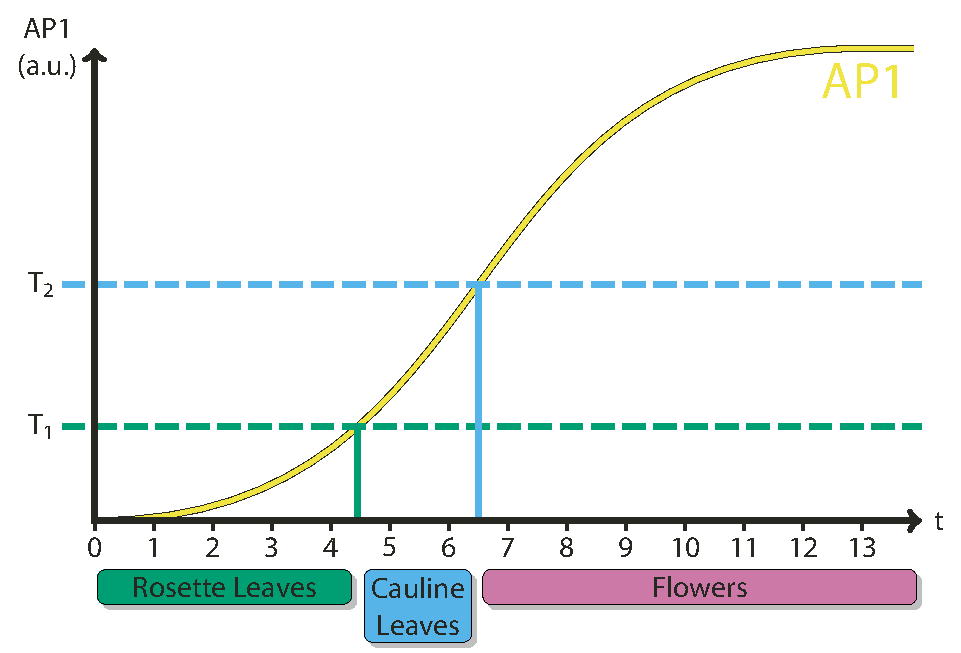
\includegraphics[width=\linewidth]{/home/nick/Dropbox/thesis/test2/sigmoid.pdf}
\caption{The definition of developmental decisions via AP1 hub levels.
An example AP1 hub curve is shown in yellow.
The developmental time taken to reach two thresholds, dashed lines, is mapped onto leaf numbers.
AP1 levels below the first threshold correspond to rosette leaves.
At the start of the transition, T\textsubscript{1}, cauline leaves are produced, and on completion of the transition, T\textsubscript{2}, flowers are made.
This mapping allows for experimental leaf number data to be used to define a cost function for inference of model parameters.
The values we used for T\textsubscript{1} and T\textsubscript{2} were 0.2 and 0.3.
a.u., arbitrary units.}
\label{fig:AP1thresholds}
\end{figure*}
After germination the first true leaves of Arabidopsis are termed rosette leaves which continue initiating during the vegetative growth phase.
We map the number of rosette leaves to the initial state and low levels of our AP1 hub.
Commencing the floral transition, lateral organs formed on the side of the bolting main shoot are termed cauline leaves.
Once the transition is complete, flowers are made.
Therefore a reliable morphological indicator of time required for initiation and length of the floral transition in the Columbia accession is the number of rosette and cauline leaves made on the main stem prior to flowers and these totals are abundantly reported throughout the literature.
To directly relate the simulated AP1 hub output to key events of the floral transition we defined two thresholds as pictured in \autoref{fig:AP1thresholds}.
The two thresholds were chosen to be at AP1 = 0.2, for the transition from rosette to cauline leaves, and at AP1 = 0.3, for the change from cauline leaves to flower production.
The decision outcome takes on one of these three states: rosette leaves, cauline leaves or flowers at these defined AP1 levels.
These threshold values are chosen arbitrarily as the parameters in the system are scaled relatively and will adjust to these selected values.
A benefit of this approach is that it can be used to quantify information on timing of both the initiation of flowering as well as the duration of the transition.
This strategy allows the developmental time to reach these states to be scaled to the leaf number data provided earlier (\autoref{tab:data}).

Having described the output of our model we now discuss the input and construction of the equations that define it.
As in the simple motifs described earlier the floral pathway integrator FT comprises a major hub for many flowering pathways.
Our model simplifies the effects of many biological and environmental processes leading to flowering by assuming they all feed in to the FT hub.
Therefore the input function to the full network model is based on FT levels.
We chose a linear time-dependent increase in FT levels until the floral transition is completed.
The transition is completed in this model when the AP1 hub threshold at 0.3 is reached and flowers are produced.
This linear with time increase of FT hub levels represents growth in leaf area proportional to time.
Further justification for this input signal is provided by the fact that the number of rosette leaves has been shown to increase at a constant rate~\cite{pouteau2009}.
The equation for the synthesis of FT is therefore $\nu_{FT}(t) = \nu_{\mathrm{FT, 35S}} + {\eta} t$, where $\eta$ is the rate of FT production per unit leaf scaled to unit time (the value chosen for this parameter was 0.01) and $\nu_{\mathrm FT, 35S}$  is the transcription rate for overexpression under the control of the 35S promoter --- if present this was taken as $1$, therefore 100 times greater than the base transcription rate in wildtype scenarios.
Genetic networks were represented by ODEs using Hill-type gene activation and repression, assuming that protein binding is in equilibrium on the timescale of translation.

\subsection{Network to Equations}

A gene network can be converted to a set of ODEs following standard practice \cite{alon2006}. 
The model includes transcriptional regulation, protein-protein interactions, and protein degradation for the hub activities in the model.
We introduce the following nomenclature.
The concentrations of the hub activity proteins are denoted by $x_1=[\mathrm{FT}]$, $x_2=[\mathrm{TFL1}]$, $x_3=[\mathrm{FD}]$, $x_4=[\mathrm{LFY}]$ and $x_5=[\mathrm{AP1}]$.
$K_{ij}$ is the effective binding constant between hub activity proteins $i$ and $j$, 
$K_{i:k}$ the effective binding constant between hub protein $i$ and a promoter site for gene $k$, 
$K_{ij:k}$ is the effective binding constant between the complex of hub activity proteins $i$ and $j$ and a promoter site for gene $k$, with $h_{i:k}$ and $h_{ij:k}$ the corresponding Hill coefficients. 
The equations governing the hub protein concentrations, $x_i$, present at any given time, $t$, are determined by the production rates, $\nu_i$, and the degradation rates, $\delta_i$, 
\begin{equation*}
\frac{dx_i}{dt}=\nu_i - \delta_{i} x_i,
\end{equation*}
in which $i=1,\ldots,5$, corresponding to FT, TFL1, FD, LFY and AP1.
The flowering time model can thus be described by differential equations, each describing the production and degradation rates for the five hubs. 
The degradation rates, $\delta_i$, were all set to a constant value, 0.1.
This can be done without loss of generality as the binding constants are allowed to change over a wide prior range to alter the effective transcription rates and adjust the effect of concentrations on downstream events. 
In reality the degradation rates are likely to differ between protein species and if the information became available these identified values can easily be substituted in to the model.

The model equations for the production rates are now discussed.
The transcription rates for the hubs are determined by the contribution from the 35S promoter, if present, $\nu_{i,\mathrm 35S}$, and a weighted sum of the rate from nothing binding to a promoter site, $\nu_{i,0}$, a singly activated level, $\nu_{i,+}$, and a doubly activated transcription rate, $\nu_{i,++}$, 
\begin{equation*}
\nu_i=\nu_{i,\rm 35S} + p_{i,0} \nu_{i,0} + p_{i,+} \nu_{i,+} + p_{i,++} \nu_{i,++}. 
\end{equation*}
The fractions, $p_i$, can be thought of as probabilities of activation and as such (including the probability of non-activation $p_{i,-}$) sum to one. 
These probabilities are determined from Hill type equations for gene activation and repression.

It is assumed that there is competitive binding between FT and TFL1 for FD~\cite{hanano2011} however this immediately complicates the equations and hence a full derivation is now given.
We assume protein-protein binding to be in equilibrium on the timescale of protein synthesis.
The total concentration of FD in the system is given by the free FD and bound FD thus $[\mathrm{FD}_{\mathrm{total}}] = [\mathrm{FD}_{\mathrm{free}}] + [\mathrm{FTFD}] + [\mathrm{TFL1FD}]$.
The concentration of FT in the system is $[\mathrm{FT}_{\mathrm{total}}] = [\mathrm{FT}_{\mathrm{free}}] + [\mathrm{FTFD}]$.
The aim is to calculate the amount of [FD] bound to [FT] and to [TFL1].
In the following we do not put square brackets, indicating concentration, or the subscripts, for clarity of presentation.
Initially, consider the concentration of FTFD and start with the assumption that free FT and FD associate at rate $k_+$ and dissociate at rate $k_-$.
Then following the law of mass-action the amount of FTFD changes over time as
\begin{equation*}
\dd{\mathrm{FTFD}}{t} = k_+\cdot \mathrm{FT}_{\mathrm{free}}\cdot \mathrm{FD}_{\mathrm{free}} - k_-\cdot \mathrm{FTFD}.
\end{equation*}
At steady state $\left(\displaystyle\dd{\mathrm{FTFD}}{t}=0\right)$ and substituting in we are left with
\begin{align*}
k_+\mathrm{FT}\left(\mathrm{FD} - \mathrm{FTFD} - \mathrm{TFL1FD}\right) &= k_-\mathrm{FTFD}, \\
\text{FTFD}\left(k_- + k_+\text{FT}\right) &= k_+\text{FT}\left(\text{FD} - \text{TFL1FD}\right),\\
\mathrm{FTFD} &= k_+\frac{\mathrm{FT}\left(\mathrm{FD} - \mathrm{TFL1FD}\right)}{k_- + k_+\cdot \mathrm{FT}}.
\end{align*}
Bringing together the binding constants in to one term, $k_d^{\mathrm{FT}}$, we are left with
\begin{equation}\label{eq:FTFDearly}
\mathrm{FTFD} = \frac{\mathrm{FT}\left(\mathrm{FD} - \mathrm{TFL1FD}\right)}{k_d^{\mathrm{FT}} + \mathrm{FT}},
\end{equation}
and by similar arguments therefore also
\begin{equation}\label{eq:TFL1FDearly}
\mathrm{TFL1FD} = \frac{\mathrm{TFL1}\left(\mathrm{FD} - \mathrm{FTFD}\right)}{k_d^{\mathrm{TFL1}} + \mathrm{TFL1}}.
\end{equation}
Substituting \eqref{eq:TFL1FDearly} into \eqref{eq:FTFDearly} as
\begin{equation*}
\mathrm{FTFD} = \frac{\mathrm{FT}}{k_d^{\mathrm{FT}} + \mathrm{FT}}\left(\mathrm{FD} - \frac{\mathrm{TFL1}\left(\mathrm{FD} - \mathrm{FTFD}\right)}{k_d^{\mathrm{TFL1}} + \mathrm{TFL1}}\right),
\end{equation*}
leaves us with
%\begin{equation}
\begin{multline*}
\left(k_d^{\mathrm{TFL1}} + \mathrm{TFL1}\right)\left(k_d^{\mathrm{FT}} + \mathrm{FT}\right)\mathrm{FTFD} = \\ \mathrm{FT}\left(\mathrm{FD}\left(k_d^{\mathrm{TFL1}} + \mathrm{TFL1}\right) - \mathrm{TFL1}\left(\mathrm{FD} - \mathrm{FTFD}\right)\right),
\end{multline*}
%\end{equation}
and after some cancelling and rearrangement
%\begin{equation}
\begin{multline*}
\left(k_d^{\mathrm{TFL1}} + \mathrm{TFL1}\right)\left(k_d^{\mathrm{FT}} + \mathrm{FT}\right)\mathrm{FTFD} - \mathrm{FT}\cdot \mathrm{TFL1}\cdot \mathrm{FTFD} = \\ k_d^{\mathrm{TFL1}}\cdot \mathrm{FT}\cdot \mathrm{FD}.
\end{multline*}
%\end{equation}
Extracting the FTFD term we are seeking and dividing across gives us
\begin{equation*}
\mathrm{FTFD} = \frac{k_d^{\mathrm{TFL1}}\cdot \mathrm{FT}\cdot \mathrm{FD}}{\left(k_d^{\mathrm{TFL1}} + \mathrm{TFL1}\right)\left(k_d^{\mathrm{FT}} + \mathrm{FT}\right) - \mathrm{FT}\cdot \mathrm{TFL1}}.
\end{equation*}
Expanding the denominator and cancelling the $FT\cdot TFL1$ term simplifies our final equation for the concentration of FT-bound FD to
\begin{equation*}
\mathrm{FTFD} = \frac{k_d^{\mathrm{TFL1}}\cdot \mathrm{FT}\cdot \mathrm{FD}}{k_d^{\mathrm{FT}}k_d^{\mathrm{TFL1}} + k_d^{\mathrm{FT}}\mathrm{TFL1} + k_d^{\mathrm{TFL1}}\mathrm{FT}}.
\end{equation*}
Analogously the equation for the concentration of FD bound to TFL1 is
\begin{equation*}
\mathrm{TFL1FD} = \frac{k_d^{\mathrm{FT}}\cdot \mathrm{TFL1}\cdot \mathrm{FD}}{k_d^{\mathrm{FT}}k_d^{\mathrm{TFL1}} + k_d^{\mathrm{FT}}\mathrm{TFL1} + k_d^{\mathrm{TFL1}}\mathrm{FT}}.
\end{equation*}
Using the previous notation
\begin{equation*}
x_{13}=x_{1}x_3 = [ \mathrm{FTFD} ]=\frac{K_{23} \cdot x_1 \cdot x_3}{K_{13}\cdot K_{23} + K_{13}\cdot x_2 + K_{23} 
\cdot x_1},
\end{equation*}
\begin{equation*}
x_{23}=x_{2}x_3 = [ \mathrm{TFL1FD} ]=\frac{K_{13} \cdot x_2 \cdot x_3}{K_{13}\cdot K_{23} + K_{13}\cdot x_2 + K_{23}
\cdot x_1}.
\end{equation*}

The transcription of \emph{TFL1} hub genes consists of a single repression rate, $\nu_{2,+}$, if one transcription factor binds and a double repression rate, $\nu_{2,++}$, with the bindings of LFY and AP1 modelled as repressing Hill functions:
\begin{equation*}
p_{5:2} = \frac{T_f^{h_{5:2}}}{T_f^{h_{5:2}}+x_5^{h_{5:2}}},
\end{equation*}
\begin{equation*}
p_{4:2} = \frac{K_{4:2}^{h_{4:2}}}{K_{4:2}^{h_{4:2}} + x_4^{h_{4:2}}},
\end{equation*}
in which $T_f$ is the threshold value of AP1 at which the plant enters the floral transition, 0.2.
Thus the transcription of \emph{TFL1} is $\nu_2 = \nu_{2, \mathrm 35S} + \nu_{2,+}\left(\left(1 - p_{5:2}\right)p_{4:2} + \left(1 - p_{4:2}\right)p_{5:2}\right) + \nu_{2,++}p_{5:2}p_{4:2} $.

As \emph{FD} is strongly upregulated during the transition~\cite{wigge2005} when floral signals such as \emph{FT} increase it is suspected it is under feedback control.
A simple explanation is that it is auto-active in this regard.
Thus the transcription of \emph{FD} hub genes consists of a base transcription rate, $\nu_{3,0}$, and an enhanced rate, $\nu_{3,+}$, when the binding of FD leads to activation.
The probability of \emph{FD} being activated through FD is
\begin{equation*}
p_{13:3} = \frac{x_{13:3}^{h_{13:3}}}
{K_{13:3}^{h_{13:3}}+x_{13}^{h_{13:3}}},
\end{equation*}
where $K_{13:3}$ is the binding constant for the FTFD complex $x_{13}$ to the promoter site of \emph{FD} ($x_3$) and $h_{13:3}$ is the corresponding Hill coefficient.
The modulator of the singly activated transcription rate of \emph{FD}, $\nu_{3,+}$, is therefore $p_{3,+}=p_{13:3}$ and the amount of base rate transcription is modulated by $p_{3,0}=1-p_{3,+}$.

The transcription of \emph{LFY} genes consists of a base transcription rate, $\nu_{4,0}$, and a singly activated rate,  $\nu_{4,+}$, when the binding of FTFD or AP1 leads to activation, and a doubly activated rate, $\nu_{4,++}$ for when both FTFD and AP1 are bound to the promoter sites of \emph{LFY}.
FTFD and TFL1FD bind competitively to one promoter site of \emph{LFY} with probabilities
%
\begin{equation*}
p_{13:4} = \frac{K_{23:4}^{h_{23:4}} \cdot x_{13}^{h_{13:4}}}
{K_{13:4}^{h_{13:4}} \cdot K_{23:4}^{h_{23:4}}+ K_{23:4}^{h_{23:4}} \cdot x_{13}^{h_{13:4}}
+ K_{13:4}^{h_{13:4}} \cdot x_{23}^{h_{23:4}}},
\end{equation*}
%
 \begin{equation*}
p_{23:4} = \frac{K_{13:4}^{h_{13:4}} \cdot x_{23}^{h_{23:4}}}
{K_{13:4}^{h_{13:4}} \cdot K_{23:4}^{h_{23:4}}+ K_{23:4}^{h_{23:4}} \cdot x_{13}^{h_{13:4}}
+ K_{13:4}^{h_{13:4}} \cdot x_{23}^{h_{23:4}}},
\end{equation*}
 %
that activate and repress the transcription, respectively. $K_{13:4}$ and $K_{23:4}$ are the binding constants for the protein complex $x_{13}$ (FTFD) and $x_{23}$ (TFL1FD) to the promoter site of the gene that codes for $x_4$ (LFY) and $h_{13:4}$ and $h_{23:4}$ are the corresponding Hill coefficients. 
AP1 also activates \emph{LFY} and this was modelled as binding to a separate promoter site (not competing with FTFD or TFL1FD), 
%
\begin{equation*}
p_{5:4} = \frac{x_{5}^{h_{5:4}}}{K_{5:4}^{h_{5:4}}+x_{5}^{h_{5:4}}}, 
\end{equation*}
%
where $K_{5:4}$ is the binding constant for the protein $x_{5}$ (AP1) to the promoter site of the gene that codes for $x_4$ (LFY) and $h_{5:4}$ is the corresponding Hill coefficient. 
Thus, for the proportion of doubly activated \emph{LFY} hub genes over time we obtain $p_{4,++} = p_{13:4} p_{5:4}$, for singly activated $p_{4,+} = p_{13:4} (1-p_{5:4}) + (1-p_{13:4} - p_{23:4}) p_{5:4}$ and for promoter sites of zero occupancy $p_{4,0} = (1-p_{13:4} - p_{23:4}) (1 - p_{5:4})$. 

Similarly the transcription of \emph{AP1} genes consists of a base transcription rate, $\nu_{5,0}$, and a singly activated rate,  $\nu_{5,+}$, when the binding of FTFD or LFY leads to activation, and a doubly activated rate, $\nu_{5,++}$ for when both FDFT and LFY are bound to the promoter sites of \emph{AP1}. FTFD and TFL1FD bind competitively to one promoter site of \emph{AP1} with probabilities 
%
\begin{equation*}
p_{13:5} = \frac{K_{23:5}^{h_{23:5}} \cdot x_{13}^{h_{13:5}}}
{K_{13:5}^{h_{13:5}} \cdot K_{23:5}^{h_{23:5}}+ K_{23:5}^{h_{23:5}} \cdot x_{13}^{h_{13:5}}
+ K_{13:5}^{h_{13:5}} \cdot x_{23}^{h_{23:5}}},
\end{equation*}
%
 \begin{equation*}
p_{23:5} = \frac{K_{13:5}^{h_{13:5}} \cdot x_{23}^{h_{23:5}}}
{K_{13:5}^{h_{13:5}} \cdot K_{23:5}^{h_{23:5}}+ K_{23:5}^{h_{23:5}} \cdot x_{13}^{h_{13:5}}
+ K_{13:5}^{h_{13:5}} \cdot x_{23}^{h_{23:5}}}. 
\end{equation*}
$K_{13:5}$ and $K_{23:5}$ are the binding constants for the protein complex $x_{13}$ (FTFD) and $x_{23}$ (TFL1FD) to the promoter site of the gene that codes for $x_5$ (AP1) and $h_{13:5}$ and $h_{23:5}$ are the corresponding Hill coefficients. 

LFY also activates \emph{AP1} hub genes and this was modelled as binding a separate promoter site (not competing with FTFD or TFL1FD), 
%
\begin{equation}
p_{4:5} = \frac{x_{4}^{h_{4:5}}}{K_{4:5}^{h_{4:5}}+x_{4}^{h_{4:5}}}, 
\end{equation}
%
in which $K_{4:5}$ is the binding constant for the protein $x_{4}$ (LFY) to the promoter site of the gene that codes for $x_5$ (AP1) and $h_{4:5}$ is the corresponding Hill coefficient. 
From this we obtain for the proportion of doubly activated LFY genes over time $p_{5,++} = p_{13:5} p_{4:5}$, for singly activated $p_{5,+} = p_{13:5} (1-p_{4:5}) + (1-p_{13:5} - p_{23:5}) p_{4:5}$, and for promoter sites of zero occupancy $p_{5,0} = (1-p_{13:5} - p_{23:5}) (1 - p_{4:5})$. 

The maximal synthesis rates are set to three values, depending on whether nothing is bound, $\nu_{i,0}$, one type of activator is present, $\nu_{i,+}$, or two types of activators are working in an AND logic activation mode, $\nu_{i,++}$. 
Production and degradation rates for the AP1 hub were chosen such that the maximal concentration is unity ($\mathrm{AP1}_{max}$ = 1) in all genotypes considered.
The complete set of equations are summarised in \autoref{tab:modelEquations}.
With no further constraints, concentrations and binding constants are not independent so we chose to vary only the binding constants and Hill coefficients in the parameter inference.
This gives a total of 19 parameters to infer.

\begin{table*}[!htbp]
\centering
\begin{tabular}{@{}l}
\toprule
Hub Protein Concentrations\\
${\displaystyle\frac{d{}x_i}{d{}t}=\nu_i - \delta_{i}  x_i}$\\
\midrule
Hub Protein-Protein Binding  \\
$x_{13} ={K_{23}  x_1  x_3}/{\left(K_{13} K_{23} + K_{13} x_2 + K_{23}  x_1\right)}$\\
$x_{23}={K_{13}  x_2  x_3}/{\left(K_{13} K_{23} + K_{13} x_2 + K_{23}  x_1\right)}$\\
\midrule
Hub Gene Activation  \\
$p_{5:2} = T_f^{h_{5:2}}/\left(T_f^{h_{5:2}}+x_5^{h_{5:2}}\right)$\\
$p_{4:2} = {K_{4:2}^{h_{4:2}}}/{\left(K_{4:2}^{h_{4:2}} + x_4^{h_{4:2}}\right)}$ \\ 
%$p_{13:2} = {K_{23:2}^{h_{23:2}}x_{13}^{h_{13:2}}} / {\left(K_{13:2}^{h_{13:2}}K_{23:2}^{h_{23:2}} + K_{23:2}^{h_{23:2}}x_{13}^{h_{23:2}} + K_{13:2}^{h_{13:2}}x_{23}^{h_{23:2}}\right)}$\\
$p_{13:3} = {x_{13}^{h_{13:3}}}/{\left(K_{13:3}^{h_{13:3}}+x_{13}^{h_{13:3}}\right)}$\\
%$p_{4:3} = {x_{4}^{h_{4:3}}}/{\left(K_{4:3}^{h_{4:3}}+x_{4}^{h_{4:3}}\right)}$\\
$p_{13:4} = {K_{23:4}^{h_{23:4}} x_{13}^{h_{13:4}}}/{\left(K_{13:4}^{h_{13:4}} K_{23:4}^{h_{23:4}}+ K_{23:4}^{h_{23:4}} x_{13}^{h_{13:4}} + K_{13:4}^{h_{13:4}} x_{23}^{h_{23:4}}\right)}$\\
$p_{23:4} = {K_{13:4}^{h_{13:4}} x_{23}^{h_{23:4}}}/{\left(K_{13:4}^{h_{13:4}} K_{23:4}^{h_{23:4}}+ K_{23:4}^{h_{23:4}} x_{13}^{h_{13:4}} + K_{13:4}^{h_{13:4}} x_{23}^{h_{23:4}}\right)}$\\
$p_{5:4} = {x_{5}^{h_{5:4}}}/{\left(K_{5:4}^{h_{5:4}}+x_{5}^{h_{5:4}}\right)}$\\
$p_{13:5} = {K_{23:5}^{h_{23:5}} x_{13}^{h_{13:5}}}/{\left(K_{13:5}^{h_{13:5}} K_{23:5}^{h_{23:5}}+ K_{23:5}^{h_{23:5}} x_{13}^{h_{13:5}} + K_{13:5}^{h_{13:5}} x_{23}^{h_{23:5}}\right)}$\\
$p_{23:5} = {K_{13:5}^{h_{13:5}} x_{23}^{h_{23:5}}}/{\left(K_{13:5}^{h_{13:5}} K_{23:5}^{h_{23:5}}+ K_{23:5}^{h_{23:5}} x_{13}^{h_{13:5}} + K_{13:5}^{h_{13:5}} x_{23}^{h_{23:5}}\right)}$\\ 
$p_{4:5} = {x_{4}^{h_{4:5}}}/{\left(K_{4:5}^{h_{4:5}}+x_{4}^{h_{4:5}}\right)}$\\
\midrule
Synthesis Rates \\
$\nu_i=\nu_{i,\mathrm 35S} + p_{i,0} \nu_{i,0} + p_{i,+} \nu_{i,+} + p_{i,++} \nu_{i,++}$\\
$p_{1,0}= 1$, $p_{1,+} = 0$, $p_{1,++} = 0$\\
$p_{2,0}= 1$, $p_{2,+} = p_{5:2}(1 - p_{4:2}) + p_{4:2}(1 - p_{5:2})$, $p_{2,++}= p_{5:2} p_{4:2}$, $T_f=0.2$\\
%$p_{3,0}=1-p_{3,+}$, $p_{3,+}=p_{4:3}$,  $p_{3,++}=0$\\
$p_{3,0}=1-p_{3,+}$, $p_{3,+}=p_{13:3}$,  $p_{3,++}=0$\\
$p_{4,0} = (1-p_{13:4} - p_{23:4}) (1 - p_{5:4})$, $p_{4,+} = p_{13:4} (1-p_{5:4}) + (1-p_{13:4} - p_{23:4}) p_{5:4}$, $p_{4,++} = p_{13:4} p_{5:4}$\\
$p_{5,0} = (1-p_{13:5} - p_{23:5}) (1 - p_{4:5})$, $p_{5,+} = p_{13:5} (1-p_{4:5}) + (1-p_{13:5} - p_{23:5}) p_{4:5}$, $p_{5,++} = p_{13:5} p_{4:5}$\\
$\nu_{1,0} = {\eta} t$, $\eta=0.01$, $\nu_{3,0} = \nu_{4,0} = 0.01$, $\nu_{2,0} = \nu_{5,0} = 0$, $\nu_{i,+}=0.05$, $\nu_{i,++} =0.1$, $\nu_{i,35S} = 1$ for $i\in\{1,\ldots,5\}$\\ 
\midrule
Initial Conditions \\
$\displaystyle\frac{\nu_{i,35S} + \nu_{i,0}}{\delta_i} $ for $i\in\{1,\ldots,5\}$\\
%$\nu_{i,35S}/\delta_i $ for $i\in\{1,2,5\}$, $\left(\nu_{i,35S} + \nu_{i,0}\right)/\delta_i $ for $i\in\{3,4\}$\\
\bottomrule
\end{tabular}
\caption{Model equations.
  The concentrations of the hub activity proteins are denoted by $x_1=[\mathrm{FT}]$, $x_2=[\mathrm{TFL1}]$, $x_3=[\mathrm{FD}]$, $x_4=[\mathrm{LFY}]$ and $x_5=[\mathrm{AP1}]$.
$K_{ij}$ are effective binding constants between hub activity proteins $i$ and $j$, 
$K_{i:k}$ the effective binding constants between hub activity protein $i$ and a promoter site for the hub activity gene $k$, $K_{ij:k}$ effective binding constants between complexes of hub activity proteins $i$ and $j$ and a promoter site for gene $k$, and $h_i$ the effective Hill coefficients.
$p_{i:k}$ is the fraction of hub activity protein $i$ bound to a promoter site of gene $k$, and $p_{ij:k}$ the fraction of the promoter of gene $k$ with the complex $i$ and $j$.
All degradation rates were set to $\delta_i=0.1$.
Initial conditions were set at $0.1$ for LFY and FD, and $0$ for the other hubs in wildtype gene scenarios.
}
\label{tab:modelEquations}
\end{table*}

\subsection{Priors for the parameters}

Uninformative priors for the parameters were chosen as we have no knowledge of their likely values \emph{in vitro} let alone \emph{in planta}.
Hill coefficients were chosen uniformly from U(1,4).
These values for Hill coefficients were also chosen in a recent DREAM challenge entry \cite{steiert2012} and are reasonable in practice \cite{sneppen2008}.
Binding coeffecients have been shown to be scale parameters \cite{grandison2008} and thus a Jeffreys-type prior was placed on those parameters with lower and upper bounds of 0.0001 and 10 respectively.

\subsection{Likelihood function}

As discussed earlier setting thresholds of the AP1 hub allows the developmental time to reach these thresholds to be scaled to leaf number data.
It is now discussed in more detail how the introduction of fixed thresholds allows for the leaf numbers to be used constructively to explore parameter space.
For all genotypes the levels of the AP1 hub are the output of our network and are mapped to the respective genotype's rosette and cauline leaf number data.
The error model was chosen to be Gaussian given the data available, \autoref{tab:data}, but as leaf numbers are integer count data a Poisson error model may be more appropriate.
The N=13 genotypes' leaf numbers in the training set are assumed to be independent with their own individual errors.
This gives a likelihood function of the form
\begin{equation*}
\mathcal L = \prod_{k=1}^N\frac{1}{\sigma_k \sqrt{2\pi}}\exp\left[\frac{-\left(f\left(\mathbf{\theta}\right)_k - \mathbf{R}_k\right)^2}{2\sigma_k^2}\right]\exp\left[\frac{-\left(f\left(\mathbf{\theta}\right)_k - \mathbf{C}_k\right)^2}{2\sigma_k^2}\right],
\end{equation*}
where $f\left(\mathbf{\theta}\right)_k$ is the function of the parameters that computes the leaf numbers. $\mathbf{R}_k$ and $\mathbf{C}_k$ are, respectively, the true rosette and cauline leaf numbers for the genotype $k$ and $\sigma_k$ the experimental standard deviation in the total leaf numbers for that genotype.
A more explicit way of writing this for our situation of evaluating the model when AP1 reaches 0.2 and 0.3, for rosette and cauline leaf numbers respectively, is the following log-likelihood function
\begin{align*}
\log\mathcal L = &-N\log\left(\sqrt{2\pi}\right) - \sum_{k=1}^N\log\sigma_k\nonumber\\ &- \sum_{k=1}^N\frac{\left(\left(\left.f\left(\mathbf{\theta}\right)_k\right|_{AP1=0.2} - \mathbf{R}_k\right)^2 + \left(\left.f\left(\mathbf{\theta}\right)_k\right|_{AP1=0.3} - \mathbf{C}_k\right)^2\right)}{2\sigma_k^2}.
\end{align*}

Having defined the data, model, prior and likelihood function we now have everything in place for a proper Bayesian treatment of the problem.
Hence the model parameters were inferred by nested sampling using the leaf number data from genotypes in the training set (wildtype, single and double mutants).
The resulting posterior distribution of the parameters for the model was used to make predictions for the triple mutants and explore the model's dynamics, sensitivity and robustness.

\section{Results}
\subsection{Biological evidence contradicts statistical evidence}

Given the data available nested sampling estimates the log evidence for the derived model to be $-56.17\pm 0.17$.
The parameters from 2000 equally-weighted posterior samples are used to give the estimated leaf numbers for all genotypes in \autoref{tab:postFDFDLeafNums}
\sidenote{\emph{Taking the parameters from the best-fit nested sample gives a maximum likelihood score of $-24.072$.
The estimated leaf numbers from this set of parameters are also given in \autoref{tab:postFDFDLeafNums}.}}
.
The network output is able to capture the true leaf numbers well for the training set and predict the triple mutant leaf numbers.
The largest predicted leaf number deviation is for the triple mutant \emph{tfl-1 fd-2 fdp-1} where the model predicts six more rosette leaves than recorded experimentally.
These inaccuracies do not surprise us.
The triple mutants were deliberately chosen as a prediction set to test the network to its fullest.
The effect of adding extra mutations is clearly not simply additive. 
The fact that our estimated leaf numbers are in the right ball park then is encouraging because we believe we have captured some of the genetic variability in our network structure.
During the undertaking of this research a paper was published \cite{winter2011} showing that FD is a target gene of LFY, at least at the seedling stage.
This could explain the observation that FD expression is strongly upregulated during the floral transition \cite{wigge2005}.
Further experiments were suggested and analysis of the FD promoter revealed it contains two LFY binding sites \cite{jaeger2013}.
It was also demonstrated that deletion of the LFY binding sites in the FD promoter abolishes FD upregulation upon the floral transition and ChIP showed that the binding was direct between LFY and the FD promoter \cite{jaeger2013}.
In light of this conclusive biological evidence we removed our hypothesised auto-activation of the FD hub which accounted for the upregulation of FD during the floral transition and replaced it with a term describing feedback from the LFY hub on to FD.
The equation for probability of FD being activated, now through LFY, becomes
\begin{equation*}
p_{4:3} = \frac{x_{4}^{h_{4:3}}}
{K_{4:3}^{h_{4:3}}+x_{4}^{h_{4:3}}},
\end{equation*}
where $K_{4:3}$ is the binding constant for LFY protein, $x_{4}$, to the promoter site of the gene that codes for $x_3$ (FD) and $h_{4:3}$ is the corresponding Hill coefficient.

\begin{table*}[!htb]
\centering
%\footnotesize
%\setlength{\tabcolsep}{3pt}
    \begin{tabular}{@{}l@{\hspace{0.8em}}ccc@{\hspace{0.5em}}c@{\hspace{1.4em}}c@{\hspace{0.7em}}c@{\hspace{0.7em}}cc@{}}
      \toprule
      Genotype  & \multicolumn{3}{c}{ No. of rosette leaves} && \multicolumn{3}{c}{ No. of cauline leaves} & Data set \\
\cmidrule(){2-4} \cmidrule(){6-8}
& True & \multicolumn{2}{c}{Model} && True & \multicolumn{2}{c}{Model} & \\
\cmidrule(){3-4} \cmidrule(){7-8}
& & Best-fit & Mean $\pm$ SD &&& Best-fit & Mean $\pm$ SD \\
%    \begin{tabular}{@{}lccccccccc@{}}
%      \toprule
%      Genotype  & \multicolumn{3}{c}{ No. of rosette leaves} && \multicolumn{3}{c}{ No. of cauline leaves} & Model set \\
%\cmidrule(r){2-4} \cmidrule{6-8}
%& Experiment & Model best-fit & Model mean $\pm$ SD && Experiment & Model best-fit & Model mean $\pm$ SD \\
      \toprule
      Wild type (Col)             & 7.9   & 8.8  &  8.7  $ \pm $  0.4  && 1.4  & 1.8  &  1.8 $ \pm $ 0.1   &  Training\\ 
      35S:\emph{FT}               & 4.4   & 4.3  &  4.1  $ \pm $  0.3  && 1.0  & 1.7  &  1.7 $ \pm $ 0.1   &  Training\\ 
      35S:\emph{LFY}              & 3.8   & 4.8  &  4.7  $ \pm $  0.1  && 1.8  & 2.1  &  2.2 $ \pm $ 0.1   &  Training\\ 
      35S:\emph{TFL1}             & 27.5  & 27.1 & 26.8  $ \pm $  1.8  && 15.7 & 15.5 & 14.4 $ \pm $ 1.9   &  Training\\ 
      \emph{lfy-12}               & 13.0  & 13.4 & 13.6  $ \pm $  0.8  && 5.3  & 4.9  &  5.1 $ \pm $ 0.4   &  Training\\ 
      \emph{ft-10}                & 36.4  & 36.7 & 37.1  $ \pm $  1.2  && 9.3  & 8.7  &  8.6 $ \pm $ 0.9   &  Training\\ 
      \emph{tfl1-1}               & 7.7   & 8.1  &  8.3  $ \pm $  0.4  && 0.4  & 1.7  &  1.8 $ \pm $ 0.1   &  Training\\ 
      \emph{fd-2}                 & 18.5  & 15.6 & 16.1  $ \pm $  1.0  && 4.63 & 3.8  &  3.7 $ \pm $ 0.3   &  Training\\ 
      \emph{fdp-1}                & 11.2  & 9.6  &  9.5  $ \pm $  0.4  && 2.0  & 1.8  &  2.0 $ \pm $ 0.1   &  Training \\
      \emph{fd-2 fdp-1}           & 32.9  & 32.1 & 31.3  $ \pm $  1.0  && 6.3  & 7.6  &  7.3 $ \pm $ 0.7   &  Training\\ 
      35S:\emph{TFL1 fd-2}        & 23.8  & 27.8 & 27.1  $ \pm $  1.9  && 8.2  & 5.2  &  5.2 $ \pm $ 0.6   &  Training \\
      \emph{tfl1-1 fd-2}          & 14.4  & 14.2 & 15.1  $ \pm $  0.8  && 4.6  & 3.7  &  3.6 $ \pm $ 0.3   &  Training \\
      35S:\emph{FT fd-2}          & 8.3   & 8.2  &  7.7  $ \pm $  0.9  && 2.4  & 2.8  &  3.0 $ \pm $ 0.4   &  Training \\
      \emph{tfl1-1 fd-2 fdp-1}    & 24.83 & 31.0 & 30.8  $ \pm $  1.1  && 6.67 & 7.5  &  7.3 $ \pm $ 0.6   &  Prediction \\
      35S:\emph{TFL1 fd-2 fdp-1}  & 31.33 & 34.2 & 34.0  $ \pm $  1.3  && 11.0 & 8.2  &  7.7 $ \pm $ 0.8   &  Prediction \\
      35S:\emph{FT fd-2 fdp-1}    & 25.8  & 26.2 & 26.3  $ \pm $  2.2  && 5.6  & 7.4  &  7.2 $ \pm $ 0.6   &  Prediction \\
      \bottomrule
    \end{tabular}
    \caption{Experimental and model leaf number data for the network with FD auto-activation.
      For each genotype the table lists the mean experimental leaf number data and estimated (for the training set) or predicted best-fit and mean $\pm$ SD values for rosette and cauline leaves.
      The best-fit values use one set of parameters and thus has no possible associated error.
      This sample is taken from all the nested samples and is the one that maximises the likelihood function the most from the final set.
      Mean and SD based on 2000 posterior samples.
      SD, standard deviation.
    }
    \label{tab:postFDFDLeafNums}
\end{table*}

Simulating this alternative network and comparing estimates of leaf number data to experimental leaf numbers reveal some differences in the training set but in sum very little.
The predictions for the triple mutants slightly favour the FD auto-regulation model but of course a full Bayesian model comparison is preferred.
Running the nested sampling algorithm with the slightly altered network architecture gave a worse log evidence score of $-62.68\pm 0.18$.
Indeed on Jeffreys' scale the Bayes factor between these two models decisively favours the original assumption that FD is an auto-activator.
How can we account for this difference between biology and statistics?
Formally the Bayes factor is only equal to the posterior odds of two models if we assume both hypotheses to be equally true.
Biologically the prior odds should favour the LFY feedback to FD model by many orders of magnitude based on the results of the experiments suggested above.
In fact given that an investigator should only define models with a reasonable verisimilitude in model space, the first hypothesis could be discounted directly.
Statistically the evidence incorporates an Occam factor \cite{mackay2003}, penalising more complex models if their fit is not substantially improved.
Comparing a basic least squares fit to the training data for the best-fitting likelihood parameters from nested sampling reveals little difference in the sum of squared errors between models, 43.1 compared to 45.7, actually in favour of the network with LFY feedback on to FD.
These numbers came from the best-fit parameter set that was found by considering the errors in the data as described by the likelihood function and then using them in a simple least-squares residual which does not consider the errors in the data.
Thus we may not want to assign much weight to this particular finding.

\begin{figure}[!htb]
\centering
% \includegraphics[height=0.35\textheight,page=6]{/home/nick/Dropbox/thesis/loops.pdf}
\includegraphics[width=0.9\textwidth,page=6]{/home/nick/Dropbox/thesis/loops.pdf}
\sidecaption[][-280pt]{New regulatory network diagram.
  This network shows all connections in the network with LFY feedback on to \emph{FD}.
  Both FT and TFL1 act through FD (small arrows) and these are shown as ovals regulating the other hubs (circles).
  FT is the input and AP1 the output of the network model.
  Filled arrowheads indicate activation and T-bars represent inhibition.
\label{fig:LFYFDdiag}}
\end{figure}

To further build an understanding of the parameter space, a simulated annealing algorithm \cite{kirkpatrick1983,goffe1994} optimising the sum of squared errors was run from a number of random starting parameter sets.
The procedure was cooled to near 0 from a starting temperature of 50, with the temperature reduction factor set at 0.85, and each exploration at a certain temperature involving 50 cycles with 20 sub-cycles.
The majority (94 out of 96 runs) of results from the initial model were near to the lowest minimum value found, 27.9.
In contrast for the new hypothesis a sole run (out of 83) was near its lowest minimum (32.0), with most (81/83) entering a wide local minima with a best fit more than double the optimal solution (around 82).
This suggests that a large amount of parameter space fits well with the FD auto-regulatory network, but not as much does with the alternative hypothesis.
This would account for a significant difference in Occam factor and can therefore help us to explain the difference in evidence results.
Ultimately the biological evidence is overwhelming for a network that has a feedback term from the LFY hub to the FD hub (depicted in \autoref{fig:LFYFDdiag}) and thus this is the model that was taken forward.

Posterior estimates of rosette and cauline leaf numbers from this newer network are shown in \autoref{fig:violinRoseCaul}.
Firstly it can be observed that we can accurately infer both types of leaf numbers with a clear idea of the uncertainty attached with those estimates or predictions.
Secondly the violin plots show (symmetrically) the distribution of our inferred leaf numbers is unimodal.
This is important because an average prediction could be the average of two, or more, predictions that are different from the experimental value.
Using a rigid methodology such as Bayesian inference allows this to be elucidated.
In this case we show that due to there being no multimodality a mean and standard deviation will give a fair summary for both the estimates and the predictions.
\begin{figure*}[!htbp]
\centering
\includegraphics[width=\linewidth]{/home/nick/Documents/multinestThesisData/LFYFD/post-leafnums/post-leaf-violin.pdf}
\caption{Estimated and predicted rosette and cauline leaf numbers for the model with LFY feedback onto FD.
2000 posterior samples were used for kernel density estimates of each genotype as a violin plot.
The x-axis positions correspond to the mean number of experimental rosette and cauline leaves.
The density estimates reveal that the predictions are unimodal.
In a perfect-fit model the violins would all be on the dark line.
}
\label{fig:violinRoseCaul}
\end{figure*}

\subsection{Dynamics of the floral transition network}

The dynamics of the wildtype network's hub proteins representing concentrations in a cell on the flanks of the apex are shown in \autoref{fig:wtDynFacet} for 2000 randomly-drawn equally-weighted posterior samples.
It can be seen that despite variability in all hubs the output hub, AP1, is under tight control.
This is not very surprising given AP1 dynamics are what constrains the likelihood function and therefore the model fitting.
FT is most variable as it approaches its steady state but in the wildtype network this has no consequence on the estimated leaf numbers.
The effect on TFL1 of being repressed is clear to see and it reaches a steady state around zero.
FD experiences the greatest delay in upregulation.
This is because it has to wait until sufficient LFY is in the system to bind and then activate it.
LFY does not accumulate immediately because there is a slight delay before the higher transcription rate is active as it needs sufficient levels of AP1 to have both promoting binding sites occupied.
AP1 transcription and translation occurs very quickly in this wildtype set-up because initial levels of LFY are present to bind to the AP1 hub promoter.
This is rapidly followed by rising FT levels which kick in to activate the higher rates of upregulation.

Throughout the time period of the floral transition strongly rising levels of the transcription factors in the network are observed.
This is in agreement with the literature~\cite{ratcliffe1998, ratcliffe1999, wigge2005}.
The behaviour of our TFL1 hub is perhaps also reflective of reality~\cite{conti2007}, at least assuming that TFL1 protein levels can be detected at a similar level to our hub levels, yet this is less clear.
Because we have modelled a cell that is poised to transition to a flower on the flanks of the apex it can be thought of as initially being in floral anlagen --- cells that form the foundations of, in this case floral, organs.
Conti \& Bradley~\cite{conti2007} show that TFL1 protein moves without its expression domain including into anlagen cells and there \emph{LFY} is expressed.
At some point these cells experience stronger floral signals and TFL1 is restricted from floral meristems.
Thus even if \emph{TFL1} mRNA is not expressed in those primordial cells at the early stages of development that this chapter focuses on, its protein product is likely to be present before declining.
This shows the early TFL1 hub dynamics in the model could be a decent description of the system.

Another point to bear in mind when critically evaluating this network's dynamics is that the input is smooth so it is not surprising that the output is smooth.
Therefore the behaviour of the network to non-monotonic input signals is investigated next along with other important dynamics representative of the floral transition to reassure ourselves that the larger network still maintains qualitative properties of the network motifs.

\begin{figure*}[!htbp]
\centering
\includegraphics[width=\linewidth]{/home/nick/Dropbox/march2014/multinest4thesis/flowering/LFYFD/post-samples/heatmap_facet_test.pdf}
\caption{2000 posterior samples of the wildtype network dynamics of the five variables.
Darker intensity indicates more samples at that concentration for each timepoint.
FT will follow the same path initially for all samples until AP1 crosses the rosette-to-cauline threshold but fans out after a while.
TFL1 is repressed as LFY and AP1 become established.
The predictive dynamics of the AP1 hub closely match each other despite the variation in the other hub proteins.
}
\label{fig:wtDynFacet}
\end{figure*}
\subsubsection{Irreversibility}
An important characteristic of the floral transition in wildtype Arabidopsis is its irreversibility.
This means that once committed to flowering the primordia can not then revert back into vegetative tissue before making floral organs.
Because FT hub mutant plants flower after a long time in suitable conditions~\cite{kim2013}, by design our network can incorporate no FT hub production term and still output flowers.
However what if there was initially FT production that was then withdrawn?
This could represent for instance a light shift experiment from long days to darkness or a construct that can inducibly knockdown FT.
This was investigated by setting the FT production term, $\nu_{FT}$, in the model to zero after a certain number of leaves had been observed.
Simulations, using the best-fit parameters, varying the length of inductive conditions are shown in \autoref{fig:irrev}.
\begin{figure*}[!htb]
\centering
\includegraphics[width=\linewidth]{/home/nick/Dropbox/march2014/multinest4thesis/flowering/figures/irrev.pdf}
\caption{The effect of FT production withdrawal on the AP1 hub.
FT is withdrawn after the indicated number of leaves and its effect on the correspondingly coloured lines for AP1 is shown.
Flowering time is judged by AP1 crossing the 0.3 threshold.
Longer times equate to delayed flowering.
The wildtype (WT) and FT-knockout (ft) scenarios are shown for comparison.
Even a small induction of FT speeds up the time to flower compared to the knockout line.
}
\label{fig:irrev}
\end{figure*}
Flowering time is judged here by AP1 crossing the 0.3 threshold.
As can be seen flowering time is identical to the wildtype if FT is stopped after a developmental time of 10 leaves, and near identical if terminated at the eight leaf stage.
Ceasing FT production after the formation of six leaves causes a slightly delayed time to flower.
On the other hand the duration of FT production has a strong effect on the timing of flowering if withdrawn early, at the two or four leaf stage.
Compared with the simulated complete lack of the FT hub (labelled ft in \autoref{fig:irrev}) flowering is still accelerated when FT production is withdrawn after the formation of only two leaves.
Once AP1 has crossed the rosette-to-cauline threshold (0.2; around the 8 leaf stage) preventing FT production has little effect on the timing of flowering.
At this point the plant is committed to flowering which is consistent with a study showing that one long day can be sufficient to cause floral commitment under certain conditions~\cite{corbesier1996}.
Thus by introducing a flowering threshold this network can exhibit irreversibility, and from earlier we know this is due to the memory element present in the core regulatory motif.

\subsubsection{Noise Filtering}

\emph{FT} expression is strongly influenced by temperature~\cite{balasubramanian2006}.
Therefore plants are likely to experience large day-to-day fluctuations in \emph{FT} levels.
To simulate these conditions first uniform random noise of up to 50\% of the signal $\nu_{FT}$ was given as input.
With this level of noise FT hub levels are only minorly perturbed, \autoref{fig:noisy} Left, with no effect on the AP1 hub.
Pushing this further very high noise levels in FT production rates were simulated such that uniform random noise of up to 200\% $\nu_{FT}$ was given as input.
These signals propagate through to the levels of FT, \autoref{fig:noisy} Right, however the network is also able to filter this out, resulting in a smooth AP1 curve.
Under these conditions the model simulates the ability of this developmental system to filter noisy environmental signals and make correctly timed decisions.
The buffering properties of the model result in AP1 levels that are unaffected by these perturbations because of the incorporated coherent feedforward loop.
\begin{figure*}[!htb]
\centering
\includegraphics[width=\linewidth]{/home/nick/Dropbox/march2014/multinest4thesis/flowering/figures/noisy.pdf}
\caption{Effect of signal noise on the network hubs.
50\% (left) or 200\% (right) random noise was added to the signal (purple).
The lower level of noise in the FT input barely filters through to the FT hub (red) thus not surprisingly the AP1 (yellow) output is smooth.
The high noise levels affect the FT hub more strongly but they are also filtered out by the network so there is no effect on the AP1 hub.
}
\label{fig:noisy}
\end{figure*}

\subsubsection{Circadian Oscillations}
Both FT hub genes \emph{FT} and \emph{TSF} are expressed in a circadian fashion \emph{in planta}~\cite{suarezlopez2001,yamaguchi2005}.
\emph{AP1} expression, our marker for the output of the flowering pathway, does not oscillate~\cite{sundstrom2006}.
We wished to test how well our full regulatory network also exhibits this ability to integrate out and smooth input signals.
Hence it was examined how oscillating production rates of FT influence the FT and AP1 hubs in particular.
The input term, $\nu_{FT}$, was multiplied by the oscillating function $\sin(ct)^2$, where c controls the frequency, either 0.5 (\autoref{fig:circ} Left) or 3 (\autoref{fig:circ} Right).
As shown in these figures the network is able to filter out large oscillations in FT production rate at both high and low frequencies.
These modulations propagate through to FT levels yet generate an unperturbed increase in AP1.

\begin{figure*}[!htbp]
\centering
\includegraphics[width=\linewidth]{/home/nick/Dropbox/march2014/multinest4thesis/flowering/figures/circ.pdf}
\caption{Effect of oscillating FT input signal on the network hubs.
Upper row: degradation rates are set at 0.1 as used throughout this chapter.
The circadian oscillations at low frequency (left) of FT activation (purple) propagate through to the FT hub (red) with no effect on the AP1 hub (yellow).
High frequency (right) FT activation oscillations transmit through to the FT hub with small amplitude and thus this does not prevent a smooth rise in the AP1 hub.
Lower row: the degradation rates are doubled to 0.2.
Very small modulations are seen at the start of the AP1 hub curve due to the massive amplitude in the FT hub's oscillations (left).
High degradation rates and fast oscillating FT input signal again damp the FT hub's dynamics without affecting AP1 (right).
}
\label{fig:circ}
\end{figure*}

As stated previously our proposed network contains a motif that is known to buffer noise well.
However in this flowering time model the ability to buffer noise is also partly a result of the magnitude of the degradation rates compared to the steady state values.
Doubling the degradation rates, such that the modulation in $\nu_{FT}$ is fed through even more strongly to FT, we still find that the network filters out these perturbations, \autoref{fig:circ} (Lower row).
The full model therefore captures key properties of the floral transition in Arabidopsis, including irreversibility and the filtering of noisy and circadian signals, due to the network motifs built into its architecture.

\subsection{Parameter analysis}

The marginal distributions of the 19 parameters over their prior range are shown in \autoref{fig:flowerMarg}, and then after zooming in on regions of non-zero probability in \autoref{fig:flowerMargZoom}.
These distributions show a number of interesting things justifying the use of a Bayesian treatment of the problem.
We note how some Hill parameters can take on most values of their prior and thus are not constrained by the data.
In constrast the data constrains some parameters very strongly.
As these distributions are correctly normalised to have an area equalling one the parameters with higher values are the ones that are most defined.
In particular the binding coefficient of LFY on to the \emph{TFL1} promoter, $K_{4:2}$, has a high probability in the region between $10^{-4}$ and $10^{-2}$.
The parameters controlling the binding coefficient of a number of species to \emph{AP1} are also well defined.
This perhaps does not surprise because the AP1 levels are the output of our system and must therefore be constrained to give a reasonable likelihood score.
No parameters seem to show multimodality in their marginal distributions, but not all have one strong peak.
This discovery might not be accounted for with classical statistical techniques.
For example the mean and standard deviation of the Hill parameter controlling the binding of the TFL1FD hub complex to \emph{AP1}, $h_{23:5}$, would completely miss the fact that more weight is given to the higher end of the parameter value, around 4. 

In fact this case highlights a strength of the Bayesian approach as it can raise a concern, leading one to investigate model reliability but providing an avenue for updating our degrees of belief.
It seems that high Hill coefficients are preferred for both $h_{23:5}$ and $h_{4:3}$, meaning that for a second round of inference maybe the prior range should be extended.
However such large Hill terms are improbable in many realistic situations.
To account for this habit of large Hill coefficients resulting from parameter inference we could either be more specific with our prior belief on the parameters by choosing a different prior distribution, or one could add a penalty to the likelihood function.
A simple prior distribution to consider here could be a triangular distribution with most weight at the end nearest one and little weight at high values of the Hill parameter.
If the data were not informative enough to overcome our prior belief then the parameters' posterior distribution would be dominated by the prior thus alleviating the problematic high Hill coefficients.
In this flowering time model uniform priors were initially chosen for all Hill parameters as we had no knowledge of their likely values.
After examining the posterior we have revealed that firstly, if the analysis was updated then two parameters ought to have different prior distributions, and secondly that our data does not constrain the choice of all parameters to realistic values.

\begin{figure*}[!htbp]
\centering
\includegraphics[width=\linewidth]{/home/nick/Dropbox/march2014/multinest4thesis/flowering/LFYFD/margAndJoints/marginalsBasic.pdf}
\caption{Estimated marginal posterior parameter distributions over prior range.
The kinetic parameters, $K_*$, have a $\log_{10}$-uniform prior range of $[10^{-4},10]$.
The Hill terms, $h_*$, follow the prior $U(1,4)$.
More kinetic parameters than Hill parameters have a higher probability density indicating they are the more constrained.
All marginals have been properly normalised with area equal to one, thus the y-axis values represent estimated probability densities.
}
\label{fig:flowerMarg}
\end{figure*}
\begin{figure*}
\includegraphics[width=\linewidth]{/home/nick/Dropbox/march2014/multinest4thesis/flowering/LFYFD/margAndJoints/marginalsZoom.pdf}
\caption{Estimated marginal posterior parameter distributions zoomed in on non-zero probability regions.
No parameters are multimodal however not all have one strong mode.
Some Hill parameters can take on most prior values with almost equal probability.
Intriguingly this applies for $h_{4:2}$ which is the Hill term for binding of LFY on to the \emph{TFL1} promoter whereas its corresponding kinetic parameter ($K_{4:2}$) is the mostly tightly controlled parameter.
Y-axis values represent estimated probability densities with marginal distribution area equal to one.
}
\label{fig:flowerMargZoom}
\end{figure*}

\begin{figure*}[!htbp]
  \centering
  \includegraphics[width=\linewidth]{/home/nick/Dropbox/march2014/multinest4thesis/flowering/LFYFD/margAndJoints/jointsZoomRandom.pdf}
  \caption{Estimated joint posterior parameter distributions for selected parameters.
    A sample of joint distributions of different parameter values gives a better understanding of parameter space.
    Brighter colours indicate higher relative probability.
    % Top row: Parameters 0 and 1; Parameters 3 and 7.
    % Middle row: Parameters 4 and 5; Parameters 8 and 12.
    % Bottom row: Parameters 10 and 15; Parameters 16 and 18.
  }
  \label{fig:flowJointRan}
\end{figure*}
\begin{figure*}[!htbp]
  \centering
  \includegraphics[width=\linewidth]{/home/nick/Dropbox/march2014/multinest4thesis/flowering/LFYFD/margAndJoints/jointsZoomCorrelated.pdf}
  \caption{Estimated joint posterior parameter distributions showing correlations.
    All joint distributions were studied and the ones presented here show the most interesting correlations between parameters.
    Joint distributions can reveal hard to uncover information about parameter space such as correlations or multimodality.
    Brighter colours indicate higher relative probability.
    % Top row: Parameters 0 and 6; Parameters 1 and 4.
    % Middle row: Parameters 1 and 7; Parameters 1 and 8.
    % Bottom row: Parameters 2 and 5; Parameters 7 and 8.
  }
  \label{fig:flowJointCorr}
\end{figure*}

A selection of joint distributions between parameters is shown in \autoref{fig:flowJointRan}.
No combinations of parameters appear multimodal although there are correlations in some combinations (\autoref{fig:flowJointCorr}).
For example, $K_{4:3}$, the parameter controlling the binding of LFY onto \emph{FD} exhibits some correlation with other parameters.
The binding constants of the two mutual activators, \emph{AP1} and \emph{LFY}, to each other show a surprising yet evident non-linear correlation (\autoref{fig:flowJointCorr} Bottom right).
Some parameter joint distributions are so spread out that they essentially look uniformly randomly distributed as in \autoref{fig:flowJointRan} (Bottom row).
These interesting figures all together show that evaluating the posterior distribution will enable one to find more information, such as the spread or correlations, that can be missed from a point estimate of the parameters.
Likewise it can be inferred that some parameters are far more sensitive to their choice than others, and thus in the future this could be an avenue for minimising the proposed model.

Additionally the effect of some parameters on the flowering time of the wildtype network was investigated qualitatively.
It was found that the interplay between $K_{13}$ and $K_{23}$ was very important.
This is intuitive as these parameters control the relative binding strength of FD to either FT or TFL1.
Tighter TFL1 binding to FD leads to delayed flowering, which can be compensated for by lowering $K_{13}$ even more, to give tighter binding between FT and FD.
The competition for FD binding is therefore critical to correct flowering time for the input but what about for the output?
Reducing values of $K_{23:5}$, controlling the binding of the TFL1FD complex on to the \emph{AP1} promoter, again leads to a delay in AP1 accumulation.
As previously this effect can be counterbalanced by decreasing the value of $K_{13:5}$ so that FTFD binds more tightly to the \emph{AP1} promoter.

Satisfyingly these results support a number of experimental studies.
The proposal that FT may interact with FD amongst others in a transcriptional complex more strongly than TFL1 to activate flowering genes~\cite{hanano2011} is endorsed by the qualitative analysis of our network.
Yeast two-hybrid assays have shown that FT interacts more strongly with FD than TFL1 in yeast~\cite{abe2005,hanano2011}.
Looking at the marginal distributions in \autoref{fig:flowerMargZoom} of the parameters controlling the same interactions, $K_{13}$ and $K_{23}$, shows that the values for $K_{23}$ are higher leading to its weaker binding to FD in our model.
These results increase the belief that the model really captures some of the biology with how the network was constructed and the statistical treatment of the problem of parameter inference.

\subsection{A hint on spatial patterning of the SAM?}

Having established a network architecture that captures the temporal dynamics of cells undergoing the floral transition we also tentatively wondered if the model might also help us understand the spatial expression patterns of the main floral meristem regulators.
This is a particularly interesting question because during development plants show sharp boundaries of gene expression in the SAM.
During the floral transition initially diffuse and variable input signals, for example FT, gradually increase over time, leading to the expression of floral meristem genes such as \emph{LFY} and \emph{AP1} on the flanks of the shoot, while the centre of the shoot has rising \emph{TFL1} expression and remains vegetative.
It was hypothesised that low initial levels of the LFY or TFL1 hubs in the model might be sufficient to determine the stable acquisition of either a flowering (high AP1) or vegetative (high TFL1) state.
Switching between these initial conditions the wildtype network has not been found to exhibit a bistable outcome between flowering or vegetative fates.
Instead, a flowering state is often reached depending on the parameters (as discussed above).

This is expected for a number of reasons.
As the temporal model has flowers as its output, as mentioned, it can be thought of as representing a cell on the flanks of the shoot apex poised to transition.
These cells transition to a high AP1 state, but they do not experience extended upregulation of TFL1, since \emph{TFL1} is repressed in floral meristems~\cite{ratcliffe1999}.
By contrast, within the centre of the shoot, \emph{TFL1} is strongly upregulated upon flowering.
\begin{marginfigure}
    \includegraphics[width=\marginparwidth]{/home/nick/Dropbox/sept2013/PLOS1REVISIONS/tanh-FT-TFL1-plot/thesis-FT-TFL1.pdf}
    \caption{Reproduction of \autoref{fig:FT-TFL1-data}.
      There is a clear positive relationship between \emph{TFL1} and \emph{FT} expression levels as determined by qPCR.
  }
  \label{fig:FT-TFL1-data-FTchap}
\end{marginfigure}
It was found after experimental discussions that \emph{TFL1} expression correlates across an entire Arabidopsis plant with the level of \emph{FT} expression as shown in \autoref{fig:FT-TFL1-data-FTchap} (exactly the same as \autoref{fig:FT-TFL1-data} in the previous chapter).
The simplest way of accounting for this behaviour in our model was to include a term for the activation of \emph{TFL1} by FTFD in the network, as shown in \autoref{fig:FTFDTFL1diag}.
\begin{marginfigure}%[!htb]
%\centering
\includegraphics[width=\marginparwidth,page=7]{/home/nick/Dropbox/thesis/loops.pdf}
%\includegraphics[width=0.9\textwidth,page=7]{/home/nick/Dropbox/thesis/loops.pdf}
%\sidecaption[][]{Enhanced regulatory network diagram.
\caption{Enhanced regulatory network diagram.  
  This network shows an additional connection between FTFD and TFL1.
  Filled arrowheads indicate activation and T-bars represent inhibition.
\label{fig:FTFDTFL1diag}}
\end{marginfigure}
Given our hub structure this need not be a direct interaction, indeed it surely involves a number of intermediaries \emph{in planta}.
In \autoref{chapter:nestedSampling} it was seen that for this data a sigmoidal model had a strong weight of evidence for it against a linear model.
This suggests we can justifiably keep the similar structure based on Hill equations in terms of hub binding for this interaction.
The addition of this connection requires four extra parameters for FTFD binding to the promoter of \emph{TFL1} as described by the following equation
\begin{equation*}
p_{13:2} = \frac{K_{23:2}^{h_{23:2}}x_{13}^{h_{13:2}}}{K_{13:2}^{h_{13:2}}K_{23:2}^{h_{23:2}}
+ K_{23:2}^{h_{23:2}}x_{13}^{h_{23:2}} + K_{13:2}^{h_{13:2}}x_{23}^{h_{23:2}}}.
\end{equation*}

To avoid complicating the model even further this term was simply multiplied by the doubly activated TFL1 rate which leads to a competition between activation through FTFD and repression from AP1 and LFY.
Hence when AP1 and LFY are present at high concentration they will be dominantly repressive over the effect of direct FTFD-induced transcription of TFL1.
The new term for TFL1 activation is then
\begin{equation*}
\begin{split}
\nu_2 = \ &\nu_{\mathrm TFL1, 35S} \\ +\ & \nu_{TFL1,+}((1 - p_{5:2})p_{4:2} + (1 - p_{4:2})p_{5:2}) \\ +\ & \nu_{TFL1,++}\cdot p_{5:2}\cdot p_{4:2}\cdot p_{13:2}.
\end{split}
\end{equation*}

\begin{table*}[!htb]
  \centering
  % \footnotesize
  \setlength{\tabcolsep}{5pt}
  \begin{tabular}{@{}l@{\hspace{0.8em}}ccc@{\hspace{0.5em}}c@{\hspace{1.4em}}c@{\hspace{0.7em}}c@{\hspace{0.7em}}cc@{}}
    \toprule
    Genotype  & \multicolumn{3}{c}{ No. of rosette leaves} && \multicolumn{3}{c}{ No. of cauline leaves} & Data set \\
    \cmidrule(){2-4} \cmidrule(){6-8}
    & True & \multicolumn{2}{c}{Model} && True & \multicolumn{2}{c}{Model} & \\
    \cmidrule(){3-4} \cmidrule(){7-8}
    & & Best-fit & Mean $\pm$ SD &&& Best-fit & Mean $\pm$ SD \\
    \toprule
      Wild type (Col)             &  7.9  & 8.9  &  8.7 $ \pm $ 0.4 &&  1.4  & 2.0 &  1.9  $ \pm $  0.09 & Training\\
      35S:\emph{FT}               &  4.4  & 3.6  &  3.8 $ \pm $ 0.2 &&  1.0  & 1.6 &  1.7  $ \pm $  0.06 & Training\\
      35S:\emph{LFY}              &  3.8  & 3.9  &  4.1 $ \pm $ 0.1 &&  1.8  & 1.5 &  1.6  $ \pm $  0.04 & Training\\
      35S:\emph{TFL1}             & 27.5  & 26.8 & 28.1 $ \pm $ 1.5 && 15.7  & 16.9& 14.3  $ \pm $  1.9 & Training\\
      \emph{lfy-12}               & 13.0  & 12.3 & 12.8 $ \pm $ 0.7 &&  5.3  & 6.2 &  6.6  $ \pm $  0.6 & Training\\
      \emph{ft-10}                & 36.4  & 35.5 & 37.0 $ \pm $ 1.4 &&  9.3  & 8.6 &  8.8  $ \pm $  1.0 & Training\\
      \emph{tfl1-1}               &  7.7  & 8.3  &  8.5 $ \pm $ 0.4 &&  0.4  & 1.9 &  1.9  $ \pm $  0.08 & Training\\
      \emph{fd-2}                 & 18.5  & 18.1 & 16.1 $ \pm $ 0.8 &&  4.63 & 3.9 &  3.4  $ \pm $  0.3 & Training\\
      \emph{fdp-1}                & 11.2  & 9.8  &  9.4 $ \pm $ 0.4 &&  2.0  & 2.2 &  2.1  $ \pm $  0.1 & Training\\
      \emph{fd-2 fdp-1}           & 32.9  & 32.8 & 31.6 $ \pm $ 0.9 &&  6.3  & 7.0 &  6.8  $ \pm $  0.6 & Training\\
      35S:\emph{TFL1 fd-2}        & 23.8  & 25.3 & 26.0 $ \pm $ 1.5 &&  8.2  & 4.5 &  4.5  $ \pm $  0.4 & Training\\
      \emph{tfl1-1 fd-2}          & 14.4  & 15.4 & 15.6 $ \pm $ 0.7 &&  4.6  & 3.4 &  3.3  $ \pm $  0.3 & Training\\
      35S:\emph{FT fd-2}          &  8.3  & 8.3  &  7.0 $ \pm $ 0.8 &&  2.4  & 3.4 &  2.8  $ \pm $  0.3 & Training\\
      \emph{tfl1-1 fd-2 fdp-1}    & 24.83 & 30.2 & 31.2 $ \pm $ 1.0 &&  6.67 & 6.6 &  6.7  $ \pm $  0.6 & Prediction\\
      35S:\emph{TFL1 fd-2 fdp-1}  & 31.33 & 34.0 & 34.9 $ \pm $ 1.1 && 11.0  & 7.2 &  7.3  $ \pm $  0.7 & Prediction\\
      35S:\emph{FT fd-2 fdp-1}    & 25.8  & 28.5 & 26.1 $ \pm $ 2.1 &&  5.6  & 6.8 &  6.6  $ \pm $  0.6 & Prediction\\ 
      \bottomrule
    \end{tabular}
    \caption{Experimental and model leaf number data for the extended network with FTFD activating TFL1.
      For each genotype the table lists the mean experimental leaf number data and estimated (for the training set) or predicted best-fit and mean $\pm$ SD values for rosette and cauline leaves.
      The best-fit values use one set of parameters and thus have no possible associated error.
      This sample is taken from all the nested samples and is the one that maximises the likelihood function the most from the final set.
      Mean and SD based on 2000 posterior samples.
      SD, standard deviation.
      \label{tab:postExtLeafNums}
      }
\end{table*}

It was tested whether this network was still capable of fitting to the leaf numbers and if so, how its Bayesian evidence ranked compared to the two models previously considered.
Running nested sampling on the same data set but with this extra connection in the model gave a log evidence of $-59.87\pm 0.18$.
The previous model, with LFY feedback on to \emph{FD}, had a log evidence of $-62.68\pm 0.18$ thus the Bayes factor is just under $3$ --- and on a normal scale is favoured $16:1$.
On Jeffreys' scale this would be strong evidence in favour of a model with this extra term despite the four additional parameters.
What is the basis for this improvement in evidence?
It is known (see \autoref{ssec:BayesModComp} and also MacKay~\cite{mackay2003}) the evidence comprises an Occam factor and a measure of goodness of fit.
Here the former should penalise our extended model requiring four more parameters, and the latter should give more accurate leaf number estimates.
Intriguingly much of the improvements come through superior estimates of mutations solely affecting the FD hub \autoref{tab:postExtLeafNums}.
The genotypes \emph{fd-2}, \emph{fdp-1} and \emph{fd-2 fdp-1} all have better estimated best-fits in the extended model, in particular the rosette leaves of the \emph{fd} mutant.
In the training set for all three network models the best-fit leaf number estimates of genotype \emph{35S:TFL1 fd-2} are the source of the poorest fits.
This suggests we haven't done as well capturing the suppression of \emph{35S:TFL1} by \emph{fd-2} as other genotypes.
In terms of predicting the triple mutant leaf numbers there are no substantial improvements or regressions.

For different parameter values, the vegetative centre of the SAM was simulated, where \emph{TFL1} is initially expressed at low levels and \emph{LFY} is absent~\cite{bradley1997,ratcliffe1998,ratcliffe1999}.
In this model scenario, rising levels of FT trigger the further upregulation of \emph{TFL1}.
The negative feedback of TFL1 onto both \emph{AP1} and \emph{LFY} prevents their expression (\autoref{fig:spatPAT} Top).
Under the opposite starting conditions, low levels of LFY and no initial TFL1, corresponding to the primordium prior to floral evocation, rising FT activates AP1 and LFY.
Since this is a positive feedback loop, high levels of AP1 and LFY are rapidly established, and TFL1 is repressed, leading to a floral state (\autoref{fig:spatPAT} Bottom).
Although no parameter sets have been found where this is a stable state --- at very high leaf numbers (when in practice the plant may have already died) this breaks down and AP1 reaches the flowering threshold --- this can be seen as a starting hypothesis that warrants future investigations.
Up until late developmental times essentially the winner takes all --- vegetative or flowering programs are established --- depending on the initial levels of either TFL1 or LFY and their sharp rise through the transition.
This simulated outcome supports the model of Ratcliffe et al.~\cite{ratcliffe1999} who suggest that one possibility for the spatial patterning is due to the relative timing of \emph{TFL1} and the floral genes' induction, and subsequent mutual inhibition in the centre or periphery of the apex.
In addition this gives us a lead to understanding the spatial patterning of the SAM where the activators of the transition must also cause a synchronous activation of their own repression in certain domains presumably due to floral signals being perceived by upstream regulators of meristem identity.
This patterning mechanism has parallels with floral induction in tomato, where the floral signal SFT upregulates a repressor of floral meristem fate in lateral meristems adjacent to floral meristems~\cite{thouet2012}.
Further understanding the system of apical patterning is an exciting goal for researchers in the future.

\begin{figure}[!htb]
\centering
% \includegraphics[height=0.35\textheight,page=6]{/home/nick/Dropbox/thesis/loops.pdf}
\includegraphics[width=\textwidth]{/home/nick/Dropbox/march2014/multinest4thesis/flowering/FTFDTFL1/spatPAT/LFY-TFL1-spat.pdf}
\sidecaption[][-300pt]{Initial conditions can determine apical cell state.
  For the timepoints shown a switch between initial conditions of LFY (green solid line) and TFL1 (blue dash-dot line) affect hub behaviour.
  Top: LFY starts at 0, TFL1 at 0.1. TFL1 is able to repress LFY and AP1 due to continued increase in FT levels.
  Bottom: Under opposite starting conditions where LFY is initially 0.1 and TFL1 is 0, LFY and AP1 are increased and flower normally while TFL1 is repressed.
\label{fig:spatPAT}}
\end{figure}

\section{Discussion}

\subsection{Strengths and limitations of the model}

A challenge to modelling complex biological systems, such as the floral transition, is that many interacting components are involved and little is known in terms of their biophysical properties such as biochemical concentrations, binding affinities for each other or half lives within the cell.
The mathematical modelling presented here thus involves considerable simplifications in terms of quantitative cell biology.
We also simplified much hard work from excellent genetic studies in Arabidopsis with the reductionist approach --- using knowledge of the major components and approximating key genes for entire hub activities.
The list of things approximated and not modelled explicitly is vast.
Therefore it is worth providing a brief list where more details are available in \autoref{sec:ftGenetics}.
In Arabidopsis a number of pathways~\cite{simpson2002,srikanth2011} converge to stimulate flowering.
This chapter focused on FT, a key floral integrator, as the input to the network.
In one fell swoop this approximated the photoperiod pathway, whose output is diurnal \emph{FT} expression; the vernalisation pathway\sidenote{\emph{Although the rapid-cycling wildtype Columbia-0 accession used as the genetic background for the genotypes in this thesis does not have this requirement.}}; and the autonomous pathway.
The age-dependent and gibberellin pathways were accounted for by gradually rising levels of the AP1 and LFY hubs.
Numerous other players in this web have been implicated: SPL transcription factors~\cite{wang2009,yamaguchi2009}, the floral integrator gene SOC1~\cite{liu2008}, hormones such as auxin~\cite{yamaguchi2013} and cytokinin~\cite{daloia2011}, various microRNAs~\cite{schmid2003}, ambient temperature~\cite{blazquez2003,kumar2012, balasubramanian2006} and the role of mechanical forces~\cite{hamant2008}.

The model was motivated by known biological interactions and the idea of using the available leaf number data to make the predictions quantitative.
This allowed us to train the network to the data and enabled the resulting model to suggest experiments that can be related back to biological entities.
We did this by defining two thresholds at effectively arbitrary values of 0.2 and 0.3.
Given the number of parameters in the model it is reasonable to believe that sensibly changing the values of these thresholds would just lead to a corresponding altering of the parameter distributions such that we still fit to the data at a similar level.
The network model is also simple enough to understand some aspects of it intuitively because of the well-studied motifs it is based on.
These advantages comes at a cost.
First, by placing the network in an ordinary differential equation framework, we need to carry out computationally costly parameter space sampling.
Although the employed nested sampling routine has been shown to perform very well for this purpose it is still true that we do not know whether or not our estimated parameter distributions are realistic or not.
Second, the reduction to activity hubs means that our individual genes do not have direct \emph{in planta} equivalents.
Despite basing our equations on kinetic binding between proteins these are actually ``hub proteins'' and therefore an approximation of the effects of different proteins in the plant.
Third, the model currently largely neglects important spatial effects.
Although we can reproduce the overall behaviour of the transition, individual interactions represent spatially averaged behaviour and conclusions from this simplified network about such details must be considered carefully.
For example we defined an appropriate network that represents well a single cell in the apex periphery that is capable of entering the transition.
A cell elsewhere in the apex may, in fact, have a different set of connections between hubs and thus experience somewhat different behaviour.

Linear modelling of the system as presented in the early part of this chapter also suffers from these limitations, and more besides.
The network approach taken here performs better than the linear model because it helps us to understand and explain dynamic behaviour.
The increase in parameters this required also gives us more flexibility in the fitting to the leaf number data.
Thus we are able to be more accurate in estimating the training genotypes along with predictions that more closely match the triple mutant data --- along with the individual rosette and cauline leaf data shown above compare \autoref{fig:TotalLeafViolin} with \autoref{fig:FTlinearIndSig} or \autoref{fig:FTlinear}.
It is also worth noting that all the network models had decisive evidence for them versus the linear model as judged on Jeffreys' scale.

\begin{figure*}[!htbp]
\centering
\includegraphics[width=\linewidth]{/home/nick/Dropbox/march2014/multinest4thesis/flowering/TOTALleafnums/post-leafnums/post-TOTAL-leaf-violin.pdf}
\caption{Posterior sampling of the extended model for total leaf numbers.
Nested sampling was run with a likelihood function that minimised the sum of the model rosette and cauline leaves against the true total leaf number.
2000 posterior samples were taken and summary statistics calculated for each genotype.
Compared with the linear models' summaries, \autoref{fig:FTlinearIndSig} and \autoref{fig:FTlinear}, these estimates and predictions are far more reflective of the real data.
We don't predict \emph{35S:TFL1 fd-2 fdp-1} as accurately as in the linear model but we are now more accurate for the entire data set.
The evidence for this model, $-47.96\pm 0.15$, is far better than the linear models' thus showing that, for this data set, the increase in parameters is quantitatively justifiable and that the network approach is considerably more powerful than linear modelling.
}
\label{fig:TotalLeafViolin}
\end{figure*}

Our model is also extensible.
Adding further hubs to this network, for example SOC1, is not too difficult and will lead to further testable hypotheses.
More expansively, models for the circadian clock~\cite{song2012} upstream of the floral transition as well as models for downstream processes such as MADS-box transcription factors specifying floral organs~\cite{vanmourik2010} could in theory all be coupled together to produce a more complete picture of floral morphogenesis at the SAM.

\subsection{Outlook}

Due to the clear mathematical foundations and robust statistical treatment of our modelling there are a number of directions this work could be expanded on in the future.
In Arabidopsis two clear paths present a fork in the road depending on what one is trying to achieve.
The main routes are either to attempt greater understanding of the detailed mechanisms involved on a simplified molecular level or to build a larger model with a greater set of features.

The first approach is the further minimisation of the presented reductionist model.
When deciding upon our hubs and their structure the aim was to capture the core essentials of the flowering time network in the most basic possible model.
However as touched upon when analysing the parameter distributions some parameters could potentially be removed from the system without loss of much flexibility.
It would then be interesting to see the smallest network that could explain the data from the floral transition.
One possibility is to remove the TFL1 hub from the network --- revisiting our initial three-node motif --- and define new equations to capture the data.
Of course we would then have to remove the plants with altered \emph{TFL1} expression from the data set, that is four out of 13 from the training set, and two of three from the prediction set.
If this path is followed using a different data set should be strongly considered.
Minimal models can help dissect complex regulation if good resolution quantitative data is available~\cite{murray2013}.
For instance a data set representing gene and protein abundance for the selected species over a number of timepoints will give far richer insights than leaf numbers alone for any flowering time modelling attempts.

The alternative path also requires a richer data set as it leads to an extended model.
As mentioned our model could be coupled with others from the literature to provide a greater understanding of floral development and patterning.
This would necessarily require some work in making sure all mathematical and biological assumptions were similar between initial models and would no doubt leave a final model with a large number of parameters.
A number of biological assumptions made in our simplification process could be reversed, perhaps independently of whether any models are chosen for coupling.
A very interesting report from Melzer et al.~\cite{melzer2008} showed, amongst other things, that in the double-mutant \emph{soc1-3 ful-2} the effect of \emph{35S:FT} on flowering is largely suppressed.
This suggests an important role for \emph{SOC1} and \emph{FUL} downstream of \emph{FT}.
How would this fit in with our hubs?
Presently our model output is the AP1 hub which reflects the activities of, at least, \emph{AP1}, \emph{CAL} and \emph{FUL} in Arabidopsis.
A recent study~\cite{balanza2014} demonstrates the likelihood of SOC1 and FUL binding as heterodimers to the promoters of their target genes such as \emph{LFY}.
Given these data perhaps the assumption that they contribute to more than one hub could be made more explicit by adding them as extra factors.
Though this of course leads to a thorny issue --- how exactly is the morphology of flowers judged?
At what point does a flower stop being recognised as such?
In our model no architectural differences between inflorescences were accounted for.
The fact that \emph{lfy} mutant inflorescences look different to \emph{ap1} mutant inflorescences~\cite{bowman1993} (of course not fogetting the amazing \emph{ap1 cal ful} cauliflower-like inflorescence) may lead to headaches when specifying the outcome of such a model.
A mention of architecture immediately brings one's thoughts to a question of space.
The current model is temporal, and the propositions here extend this to tracking the dynamic behaviour of more proteins, and perhaps mRNAs, over time.
Ultimately these genes are all interacting and possibly diffusing in the apex over time, and connections published in the literature may not be true for all cell types at all timepoints.
This therefore highlights the need for future work in Arabidopsis, as the model dicot plant species, to ultimately focus on spatial cell-based models that account for the differential expression patterning of the key floral genes.
Relevant experiments to inform these models would therefore include investigating the spatial and temporal dynamics of the relevant genes and proteins through techniques such as live imaging microscopy, laser microdissection and RNA sequencing throughout the initiation of the floral transition.
